\documentclass[
	%parspace, % Add vertical space between paragraphs
	%noindent, % No indentation of first lines in each paragraph
	%nohyp, % No hyphenation of words
	%twoside, % Double sided format
	%draft, % Quicker draft compilation without rendering images
	%final, % Set final to hide todos
]{elteikthesis}[2024/04/26]

% The minted package is also supported for source highlighting
% See elteikthesis_minted.tex for example
%\usepackage[newfloat]{minted}

% Toggle: set \UPMtrue for UPM submission, \UPMfalse for ELTE
\newif\ifUPM
\UPMtrue % change to \UPMtrue for UPM university submission

% Document's metadata
\title{Lane Boundary Extraction from High-Density LiDAR Point Clouds for HD Mapping} % title
\date{2026} % year of defense

% Author's metadata
\author{Haála Kada Iván}
\degree{Data Science MSc}

% Supervisor(s)' metadata
\ifUPM
	\supervisor{Alberto Mozo, Full Professor} % internal supervisor's name and title
	\affiliation{Mathematical Modeling and Biocomputing Group, Universidad Politécnica de Madrid} % internal supervisor's affiliation
\else
	\supervisor{Hajder Levente, Habil. Associate Professor} % internal supervisor's name and title
	\affiliation{Institute of Computer Science, Department of Algorithms and Their Applications, Eötvös Loránd University} % internal supervisor's affiliation
\fi
\extsupervisor{José Daniel Padrón, PhD} % external supervisor's name
\extaffiliation{Data Science, Maps Advanced Analytics, TomTom N.V.} % external supervisor's affiliation

% University's metadata
\ifUPM
	\university{Universidad Politécnica de Madrid} % university's name
	\faculty{Escuela Técnica Superior de Ingenieros Informáticos} % faculty's name
	\department{} % department's name (required; leave empty if not applicable)
	\city{Madrid} % city
	\logo{upm_logo} % logo
	\logotwo{etsiinf_logo} % second logo
\else
	\university{Eötvös Loránd University} % university's name
	\faculty{Faculty of Informatics} % faculty's name
	\department{} % department's name (required; leave empty if not applicable)
	\city{Budapest} % city
	\logo{elte_cimer_szines} % logo
\fi

% Add bibliography file
\addbibresource{elteikthesis.bib}

% The document
\begin{document}

% Set document language
%\documentlang{hungarian}
\documentlang{english}

% List of todos (not in the final document)
%\listoftodos[\todolabel]

% Title page (mandatory)
\maketitle
% Topic declaration page (mandatory) - can also be attached instead
%\includepdf{topicdeclaration.pdf}

% Abstract
\chapter*{Abstract}
\addcontentsline{toc}{chapter}{Abstract}
This thesis presents a geometry-based offline processing pipeline for extracting vectorized lane boundary geometries from high-density mobile LiDAR point clouds for High Definition (HD) mapping applications.
The proposed framework addresses the challenge of generating accurate lane-level ground truth data for HD map validation without relying on rasterized representations or large-scale annotated training datasets.
Since the provided LiDAR data lacked vehicle trajectory information, four trajectory reconstruction algorithms were developed and evaluated, including a novel Pulse Line Intersection method exploiting the LiDAR packet structure.
The pipeline further combines spatial binning, ground segmentation, intensity-based lane marking extraction, road surface detection, and sliding-window curve fitting to reconstruct continuous lane geometries directly from raw point clouds.
Experimental evaluation on approximately 10\,km of highway LiDAR data demonstrates that the proposed methods can reliably extract both solid and dashed lane boundaries while preserving centimetre-level geometric fidelity.
The resulting vectorized lane representations enable scalable and precise cross-section-based HD map validation workflows.
\cleardoublepage

% Table of contents (mandatory)
\tableofcontents
\cleardoublepage

% Main content
\chapter{Introduction}
\label{ch:intro}

\section{Motiváció}
\label{sec:motivation}

A térképek eredetileg emberi navigációs célokra készültek. A korai térképek jellemzően kézi rajzolással készültek, ahol a geometriai pontosság erősen függött a méretaránytól és a rajzolási konvencióktól. Egy ilyen reprezentációban akár egy ceruzavonal vastagságnyi eltérés is több tíz vagy akár száz kilométeres valós bizonytalanságot jelenthetett.

A térképkészítés digitalizációja jelentős előrelépést hozott, mivel lehetővé tette a folyamatos skálázhatóságot és a geometriai pontosság növelését. A modern digitális térképek (pl.\ GPS-alapú rendszerek) már műholdas és szenzoros mérésekre támaszkodnak, azonban ezek a rendszerek továbbra is hordoznak mérési bizonytalanságokat, illetve nem minden térképi pont esetében áll rendelkezésre közvetlen mérés, ami lokális geometriai torzulásokhoz vezethet.

Ezek a térképek elsősorban általános felhasználási esetekre készülnek, például:
\begin{itemize}
    \item emberi navigáció,
    \item helyek keresése és POI-alapú szolgáltatások,
    \item útvonaltervezés és közlekedési információk,
    \item turisztikai és location-based szolgáltatások,
    \item előzetes tervezési feladatok,
    \item alacsony--közepes pontosságot igénylő mérnöki alkalmazások.
\end{itemize}

Ezen alkalmazások többsége nem igényel méteresnél finomabb pontosságot. Például az OpenStreetMap adatok pozicionális pontosságát több tanulmány is körülbelül 1--2 méteres nagyságrendbe sorolja, azonban ez erősen regionálisan változó, mivel crowdsourced adatbázisról van szó~\cite{osmaccuracy}.

Összehasonlításképpen egy autópálya sáv szélessége jellemzően ${\sim}3{,}5$ méter, így egy átlagos 1--2 méteres térképi hiba a sáv geometriájának akár jelentős részét is lefedheti, ami már nem elfogadható olyan alkalmazásoknál, ahol sávszintű döntések szükségesek.

Ezzel szemben az autonóm járművek és fejlett vezetéstámogató rendszerek (ADAS) már nagyságrendekkel pontosabb térképi reprezentációt igényelnek. A HD (High Definition) térképek célja, hogy centiméteres pontosságú geometriai és szemantikus információkat biztosítsanak a jármű lokalizációjához és tervezéséhez.\todo{citation needed}

A HD térképek lehetővé teszik, hogy a jármű ne kizárólag a valós idejű szenzoradatokra támaszkodjon, hanem egy előre felépített, nagy pontosságú térképi reprezentációt is használjon a lokalizáció és tervezés támogatására. Ez különösen fontos olyan helyzetekben, ahol a szenzoros észlelés korlátozott, például takart látómező esetén (pl.\ nagy járművek mögötti rejtett objektumok), vagy rossz időjárási körülmények között.\todo{ide érdemes egy konkrét AV perception / occlusion paper}

A HD térképek egyik ipari példája a TomTom által fejlesztett Orbis Map rendszer, amely több rétegből álló nagy pontosságú térképi infrastruktúrát biztosít. A TomTom egy holland location technology vállalat, amely HD térképeket és kapcsolódó szolgáltatásokat nyújt autógyártók és mobilitási cégek számára.\todo{TomTom / Orbis Map citation needed}

Az Orbis Map felépítéséhez különböző adatokat használnak, melyek adatszerzési költségükben és pontosságukban is eltérnek. Például SDO (Sensor Derived Observations) és egyéb szenzoros és térképi adatokat, amelyek lehetnek saját gyűjtésűek vagy külső partnerektől származók. A térkép egyik kulcsrétege a HD Basemap, amelynek célja a sávgeometriák és úthálózati elemek centiméteres pontosságú reprezentációja, jellemzően ${\sim}10$--20 cm-es geometriai hibahatárral.

A vállalat HD Basemap rétegének előállítása többféle adatforrás és feldolgozási lépés kombinációjával történik. A legnagyobb pontosságú adatokat a MoMa (Mobile Mapping) rendszer biztosítja, amely LiDAR szenzorokkal, panorámakamerákkal, GNSS-szel és inerciális mérőegységekkel felszerelt mérőjárműveket használ. A LiDAR pontfelhőkből előállított LRI (Linear Referencing Images) és LBEM (LiDAR Bird's Eye Mosaic) reprezentációk lehetővé teszik az útfelfestések és sávszegélyek nagy pontosságú detektálását. Az LBEM egy felülnézeti, raszterizált 2D reprezentáció, amely a MoMa LiDAR pontfelhőinek talajsíkra történő vetítésével készül. Az előállítás során a MoMa jármű LiDAR méréseket, trajektória- és kalibrációs adatokat gyűjt, majd az egyes pixelek egy adott méretű (tipikusan 5 cm felbontású) térbeli cellába eső lézerpontok statisztikai jellemzőit reprezentálják.

\begin{table}[h]
    \centering
    \footnotesize
    \caption{A MoMa és SDO adatforrások összehasonlítása.}
    \label{tab:moma_sdo}
    \begin{tabular}{|p{2.5cm}|p{5.5cm}|p{5.5cm}|}
        \hline
        & \textbf{MoMa (Mobile Mapping)} & \textbf{SDO} \\
        \hline
        \textbf{Vehicles} &
        TomTom's own survey vans with high-end sensor rigs ($360^\circ$ Ladybug cameras, LiDAR/Velodyne, precision GNSS/IMU) &
        Consumer/fleet vehicles with simpler sensors (typically front-facing ADAS camera, e.g.\ MobileEye) \\
        \hline
        \textbf{A ``session''} &
        One continuous recording run by a MoMa van, producing panoramic imagery, LiDAR point clouds, and precise trajectories &
        One drive's worth of sensor-derived feature observations (signs, lanes, road borders) --- not raw imagery \\
        \hline
        \textbf{Quality} &
        Survey-grade accuracy with PPK post-processing; serves as \textbf{ground truth} &
        Lower individual accuracy (elevation drift, miscategorized signs, no heading on some features) --- but improved through aggregation across many passes \\
        \hline
        \textbf{Scale} &
        Limited to where TomTom schedules collection drives &
        Massive --- hundreds of millions of observations daily across many countries from production vehicle fleets \\
        \hline
        \textbf{Primary use} &
        High-quality map production, ground-truth validation, traffic light/sign observation creation (Rajali) &
        Broad coverage map updates, change detection, speed limit updates, lane data at scale \\
        \hline
    \end{tabular}
\end{table}

A MoMa rendszer ugyan centiméteres pontosságot biztosít, azonban globális skálán rendkívül költséges lenne kizárólag ilyen precíziós mérésekre támaszkodni. Emiatt a HD Basemap jelentős része SDO és egyéb, alacsonyabb költségű, nem precíziós mérési források felhasználásával készül. Az SDO kameraközpontú megközelítést alkalmaz, amely stereo kamerák, vizuális odometria és mélytanuló modellek segítségével nyer ki útelemeket a képi adatokból. Ez a megoldás lényegesen jobban skálázható, így lehetővé teszi a térképi lefedettség kiterjesztését nagy úthálózatokra és globális szintre.

A HD Basemap előállítása egy többlépcsős, coarse-to-fine pipeline mentén történik. Első lépésként a különböző forrásokból származó adatokat közös koordinátarendszerbe illesztik, amelyhez LiDAR-alapú source-to-source alignment és SLAM technikákat alkalmaznak. Ezt követi a perception réteg, ahol mélytanuló modellek detektálják a sávhatárokat, útfelfestéseket és egyéb közlekedési elemeket a LiDAR és kameraképek alapján. Az így kinyert geometriai elemeket egy fusion komponens egyesíti, amely bipartite matching algoritmusokkal és megbízhatósági súlyokkal kombinálja a különböző forrásokból származó megfigyeléseket.

A végső HD lane modell előállításához a rendszer az SD (Standard Definition) térképi topológiát használja kiindulási alapként, amelyet a pontosabb szenzoros megfigyelésekkel finomít. Az automatizált folyamatot a HAPT (Human Assisted Production Tooling) támogatja, ahol operátorok manuálisan ellenőrzik és javítják a bizonytalan eseteket. Az eredmény egy nagy pontosságú HD Basemap réteg, amely tartalmazza a sávgeometriákat, útfelfestéseket és egyéb lane-level közlekedési információkat.

Az így előállított HD térképek minőségét többféle metrika segítségével ellenőrzik annak érdekében, hogy megfeleljenek az elvárt pontossági követelményeknek. A legfontosabb mérőszámok közé tartozik az \textit{Absolute Positional Accuracy} (APA) és a \textit{Relative Positional Accuracy} (RPA), amelyek a sávhatároló geometriák pontosságát vizsgálják egy manuálisan előállított ground truth adatbázis segítségével.

A validáció során előre meghatározott helyeken az út irányára merőleges szakaszokat, úgynevezett \textit{cross-section}öket definiálnak. Ezeket a cross-section vonalakat az annotátorok geo-hivatkozott LBEM képekre vetítik rá, majd megjelölik azokat a pontokat, ahol a vonal metszi a sávhatárokat. A jelölések nemcsak fizikai útburkolati jelekhez tartozhatnak, hanem virtuális sávhatárokhoz is --- például szaggatott vonalak vagy részben hiányzó felfestések esetén. Így minden cross-sectionhöz egy ground truth pontkészlet tartozik.

A HD Basemap validációja során ugyanezen cross-sectionök és a térképen tárolt sávhatároló geometriák metszéspontjait is meghatározzák. A ground truth és a térképi metszéspontok összehasonlításából számíthatók az APA és RPA metrikák. Az APA a sávhatárolók abszolút eltérését méri a valós világhoz képest, míg az RPA a sávszélességek pontosságát vizsgálja, vagyis azt, hogy a szomszédos sávhatárolók közötti távolság mennyire egyezik a valósággal.

A ground truth adatbázis előállítása azonban több problémát is felvet. Egyrészt az LBEM reprezentáció LiDAR pontfelhőből származó raszteresített képként jön létre, amely esetén a pontfelhő pixelesítése információvesztéssel és geometriai pontatlanságokkal járhat. Másrészt a manuális annotáció jelentős emberi erőforrást igényel, ezért idő- és költségigényes folyamat. A szakirodalomban kimutatták, hogy még egyszerű annotációs interfész-módosítások is jelentős hatékonyságnövekedést eredményezhetnek: például az \textit{Extreme Clicking} megközelítésben előre generált javaslatok nélkül is akár ötszörös gyorsulást értek el a hagyományos bounding box annotációhoz képest~\cite{papadopoulos2017extreme}.

A dolgozatban bemutatott megközelítés erre a problémára kíván megoldást adni egy előre összefűzött LiDAR pontfelhőket feldolgozó pipeline segítségével. A cél a sávhatárolók közvetlen, vektoros reprezentációjának előállítása, amely lehetővé teszi a cross-sectionök és a sávhatároló geometriák metszéspontjainak automatikus meghatározását. Ennek eredményeként a ground truth pontok automatikusan generálhatók lennének, így az annotátorok feladata a javasolt pontok ellenőrzésére és szükség szerinti javítására korlátozódna. Ez jelentősen csökkentheti a manuális annotáció költségét és növelheti a validációs folyamat skálázhatóságát.

\cleardoublepage

\chapter{Related Works}
\label{ch:lit}

High-definition (HD) map generation has evolved into a broad research domain driven by the rapid development of autonomous driving, mobile mapping, robotics, and geographic information systems (GIS), all of which require highly detailed and accurate spatial representations. Since HD mapping combines sensing, perception, geometric processing, and semantic vectorization, the field cannot be categorized along a single dimension. Instead, the literature is commonly organized according to several overlapping perspectives, including the level of automation, methodological paradigm, temporal processing strategy, sensing modality, point cloud representation, and vectorization methodology. These categories are often interconnected; for example, a system may simultaneously be automated, LiDAR-based, offline, and geometry-driven. The following sections summarize the major taxonomic groups and review representative state-of-the-art approaches within each category.

It is also important to note that many related works focus primarily on semantic segmentation rather than precise geometric reconstruction. Some approaches perform semantic segmentation of LiDAR point clouds without producing vectorized map representations~\cite{ExtractionClassificationRoadMarkings}. Other methods vectorize road markings along their boundaries but do not reconstruct complete lane geometries~\cite{isprs-archives-XLII-2-W13-1089-2019}. In contrast,~\cite{Eisemann_2024} proposes an industrial-scale HD mapping framework relying heavily on OpenStreetMap (OSM) priors; however, the global positional accuracy of OSM data is generally insufficient for survey-grade highway mapping applications.

\section{Manual and Automated HD Mapping}
\label{sec:manual_automated}

One of the most fundamental distinctions in HD mapping concerns the degree of human involvement in the mapping workflow. Traditional HD map production pipelines are largely manual or semi-manual~\cite{rong2020lgsvlsimulatorhighfidelity}. These systems rely on dedicated survey vehicles equipped with high-precision LiDAR, GNSS, IMU, and camera systems, followed by extensive human annotation of lanes, road markings, and infrastructure elements. While such workflows provide extremely high accuracy and consistency, they are expensive, time-consuming, and difficult to scale to continental road networks or rapidly changing environments.

Consequently, recent research has increasingly shifted toward automated HD map generation. Automated systems extract road geometry and semantic information directly from sensor observations using algorithmic or machine learning-based approaches, thereby minimizing human intervention. This transition is primarily motivated by the scalability requirements of autonomous driving, where maps must be updated frequently and cost-effectively. Crowdsourced mapping frameworks further reduce acquisition costs by utilizing sensors mounted on everyday vehicles instead of dedicated survey fleets.

Current automated HD mapping systems demonstrate substantial progress in lane extraction, road boundary estimation, and vector map generation. However, fully automated approaches still face challenges related to robustness, occlusion handling, inconsistent road markings, and generalization across diverse environments~\cite{OcclusionHandlingSDMapFusion}. As a result, many industrial solutions continue to incorporate manual verification stages even when the extraction itself is largely automated.

\section{Geometric and Deep Learning-Based Approaches}
\label{sec:geometric_dl}

Another major categorization distinguishes between classical geometric methods and modern deep learning-based approaches. Geometric methods rely on explicit mathematical modeling and spatial reasoning. Typical techniques include RANSAC-based plane fitting, spline approximation, Hough transforms, clustering, and multi-view reconstruction~\cite{isprs-archives-XLII-2-W13-1089-2019}. These methods are interpretable and often independent of training data, making them attractive in applications where reproducibility and physical consistency are essential.

In contrast, deep learning approaches formulate HD mapping as a perception problem. Neural networks learn to infer lanes, intersections, and road topology directly from sensor observations. Recent transformer-based architectures, including MapTR, have demonstrated end-to-end semantic HD map generation capabilities~\cite{mapTR}. Recent deep learning frameworks employ increasingly sophisticated architectures for vectorized HD mapping, including multi-granularity attention mechanisms and generative diffusion models for robust road geometry reconstruction and uncertainty estimation~\cite{yang2024mgmapnetmultigranularityrepresentationlearning, monninger2025mapdiffusiongenerativediffusionvectorized}.
These methods are typically trained on large-scale annotated datasets and can model highly complex urban road networks.

Despite their success, learning-based methods remain strongly dependent on training data quality, annotation consistency, and sensor configurations. They may also generalize poorly when applied to environments significantly different from the training domain. Geometric methods, while generally less adaptive and often requiring manual parameter tuning, provide greater transparency and deterministic behavior. An additional advantage is that they do not require massive annotated datasets or computationally expensive training procedures. This consideration is particularly important in the present work, where the lack of large-scale labeled data directly motivates the use of a geometry-driven pipeline.

\section{Online and Offline Mapping Pipelines}
\label{sec:online_offline}

HD mapping systems can also be categorized according to whether map generation is performed online or offline. Offline approaches process sensor data after acquisition, allowing computationally intensive optimization and globally consistent reconstruction. Such workflows commonly employ Simultaneous Localization and Mapping (SLAM), loop-closure optimization, batch point cloud registration, and high-resolution vector fitting~\cite{eightpopularLidarandVisualSLAM}. Offline systems prioritize geometric accuracy and completeness over latency.

Online HD mapping, in contrast, aims to generate local maps in real time directly onboard the vehicle. This paradigm has become increasingly important for autonomous driving systems that must react dynamically to temporary road changes, construction zones, and evolving traffic conditions. Online systems typically operate on local regions surrounding the vehicle and employ lightweight sensor fusion and incremental update strategies to satisfy strict runtime constraints. Pretrained models continuously infer local HD maps relative to the vehicle during operation~\cite{li2022hdmapnetonlinehdmap}.

Current state-of-the-art online approaches primarily rely on deep neural networks and bird’s-eye-view (BEV) representations to enable rapid inference from sequential sensor data. However, limited computational resources and the absence of long-range optimization often reduce global consistency and geometric precision. Therefore, in applications requiring survey-grade accuracy and highway-scale consistent vector maps, offline approaches remain dominant.

\section{Categorization by Sensor Modality}
\label{sec:sensor_modality}

HD mapping methods may additionally be categorized according to their primary sensing modality. Camera-based approaches use RGB imagery to infer lane boundaries, road markings, and semantic context. These methods benefit from rich texture information and relatively inexpensive hardware. However, purely image-based systems suffer from perspective distortion, limited depth estimation accuracy, and sensitivity to illumination and weather conditions~\cite{li2022bevformerlearningbirdseyeviewrepresentation}.

Large-scale road network segmentation from aerial imagery has also been explored using OpenStreetMap-based supervision~\cite{ParsingAerialImagesAroundtheWorld}. However, the work focuses on semantic road extraction rather than HD map generation.

LiDAR-based approaches instead rely on dense 3D point clouds and reflectance measurements. LiDAR provides highly accurate geometric information and naturally supports metric bird’s-eye-view processing. Furthermore, LiDAR intensity values can reveal lane markings and painted road patterns even under poor lighting conditions. Consequently, LiDAR has become one of the dominant sensing modalities in HD mapping research~\cite{gong2024lidarbasedhdmaplocalization}.

Fusion-based approaches combine LiDAR and camera data to exploit the strengths of both modalities. Camera images provide semantic richness and visual context, while LiDAR contributes precise geometry and depth information. Recent multimodal fusion architectures demonstrate improved robustness and extended perception range. Nevertheless, fusion systems require careful calibration and synchronization, and their performance may degrade significantly when one sensing modality becomes unreliable or unavailable~\cite{HDMapFusion}.

Current research trends increasingly emphasize multimodal fusion, particularly in urban autonomous driving scenarios.

\section{Point Cloud Representation Strategies}
\label{sec:point_cloud_repr}

In LiDAR-based mapping systems, another important distinction concerns how the point cloud itself is represented and processed. One major category converts 3D LiDAR data into image-like representations. Bird’s-eye-view (BEV) projections discretize points into top-down occupancy or intensity grids, enabling the application of conventional convolutional neural networks. Similarly, range-image representations project LiDAR points into spherical coordinates aligned with the sensor scanning pattern. These representations simplify learning but introduce discretization artifacts~\cite{wu2017squeezesegconvolutionalneuralnets}.

An alternative strategy processes raw point clouds directly. Point-based neural architectures operate directly on unordered point sets without projection, thereby preserving geometric fidelity~\cite{qi2017pointnetdeeplearningpoint, thomas2019kpconvflexibledeformableconvolution, hu2020randlanetefficientsemanticsegmentation}. These methods preserve full geometric fidelity and avoid information loss caused by rasterization. However, they are computationally expensive and difficult to scale to very large scenes~\cite{qi2017pointnetdeeplearningpoint, thomas2019kpconvflexibledeformableconvolution, hu2020randlanetefficientsemanticsegmentation}.

Voxel-based and point-pillar-based methods attempt to balance efficiency and geometric expressiveness. Voxel-based and point-pillar-based methods attempt to balance computational efficiency and geometric expressiveness through structured spatial discretization~\cite{graham20173dsemanticsegmentationsubmanifold, lang2019pointpillarsfastencodersobject}. These approaches achieve favorable runtime characteristics and have become widely adopted in autonomous driving perception systems.

Recent research trends increasingly favor hybrid representations that combine efficient spatial discretization with adaptive local feature extraction. Nevertheless, purely geometric offline processing pipelines often continue to operate directly on raw point clouds in order to preserve accuracy and avoid discretization artifacts during vectorization~\cite{liu2019pointvoxelcnnefficient3d}.

It should be noted that many of the above references originate from the broader fields of LiDAR perception and geometric processing rather than HD map generation specifically. However, these methods constitute the foundational building blocks of modern LiDAR-based HD mapping systems, where segmentation and detection techniques are extended into globally or locally consistent spatial representations.

\section{Geometric and Spatial-Statistical Vectorization Approaches}
\label{sec:geometric_vectorization}

In the present work, the input consists of a pre-georeferenced mobile LiDAR point cloud. Since no large-scale annotated dataset is available for supervised learning, the proposed solution follows an offline, geometry-driven LiDAR processing pipeline.

These approaches focus on directly extracting structured road representations from geometric and reflectance information without relying on machine learning.

A common strategy is trajectory-driven region-of-interest clipping. Here, the reconstructed vehicle trajectory defines the processing corridor, allowing algorithms to focus exclusively on points near the roadway while filtering out irrelevant environmental structures. This significantly reduces computational complexity and improves robustness. Consequently, trajectory reconstruction becomes an important component of the proposed pipeline, although this step is omitted in existing HD mapping workflows where accurate trajectories are assumed to be already available.

Ground segmentation represents another fundamental stage. Classical approaches commonly employ RANSAC-based plane fitting, rasterization followed by region growing, or local surface estimation techniques to separate the road surface from surrounding infrastructure and vegetation~\cite{Ground_image-basedsegmentation, Segmentationof3Dlidardatainnonflaturbanenvironments}. One approach first removes a large portion of non-ground points by analyzing distances and inclination angles between consecutive LiDAR rings, followed by RANSAC-based extraction of the remaining ground surface~\cite{interringground}. Nevertheless, handling curved roads, abrupt elevation changes, and environments containing multiple local planes remains an active research challenge.

After ground extraction, road markings are typically identified using intensity-based segmentation. These methods exploit the higher reflectivity of painted lane markings compared to asphalt surfaces. A simple but commonly used heuristic considers points belonging to the upper intensity percentiles as candidate road markings. More adaptive histogram-based thresholding techniques include Otsu and Kapur maximum-entropy thresholding methods~\cite{otsu1979threshold, GUAN201493, isprs-archives-XLII-2-W13-1089-2019}.

Although such heuristic methods perform well in controlled environments such as highways with relatively uniform road paint quality, they often produce large numbers of false positives under low-intensity contrast conditions, for example on concrete road surfaces~\cite{IntensityThresholdingandDeepLearningBasedLaneMarkingExtraction}. Modern online HD mapping systems increasingly employ deep learning-based semantic segmentation approaches instead. Architectures based on PointNet++, transformers, and related models utilize not only intensity but also geometric and spatial context, enabling more robust detection of degraded lane markings in complex urban environments.

In the proposed pipeline, this stage is implemented using either Kapur thresholding or percentile-based thresholding as configurable alternatives.

The final vectorization stage generally involves curve fitting and topological reconstruction. Polynomial curves, B-spline interpolation, clothoid (Euler spiral) approximations, and Moving Least Squares (MLS) smoothing are commonly applied to generate continuous lane geometries compatible with HD mapping standards. Clothoid models are particularly popular in autonomous driving HD maps because they provide linearly varying curvature, closely matching real-world road design principles and vehicle dynamics models~\cite{RoadNetworkGenerationTechniquesReview}. Beyond geometric accuracy, vectorization must also ensure topological consistency, including lane connectivity, splits, and merges. The primary objective of such approaches is to produce geometrically continuous and physically realistic lane models while maintaining compact and efficient map representations for autonomous navigation systems.

Although deep learning-based approaches currently dominate many benchmark evaluations, geometric vectorization methods remain highly relevant in survey-grade offline mapping due to their interpretability, deterministic behavior, and compatibility with engineering road models. Furthermore, geometric pipelines do not require large annotated training datasets or computationally expensive model training procedures.

\section{Benchmark Datasets and Coordinate Systems}
\label{sec:datasets}

Research in HD mapping is also strongly influenced by the characteristics of available benchmark datasets. Widely used datasets such as nuScenes, Waymo Open Dataset, Argoverse, ApolloScape, and KITTI-360 typically employ egocentric or city-specific coordinate systems~\cite{nuscenes, mei2022waymoopendatasetpanoramic, argoverse, apolloscape, kitti-360}. These datasets were primarily designed for autonomous driving perception tasks and therefore emphasize local consistency rather than globally accurate georeferencing.

While these datasets are extremely valuable for learning-based perception research, they are less suitable for large-scale georeferenced mapping workflows. Absolute coordinate consistency is often limited, and integration with GIS systems or infrastructure databases may require additional alignment procedures.

Globally georeferenced LiDAR datasets suitable for highway-scale HD mapping remain relatively rare. Existing datasets with GPS/IMU integration frequently lack dense lane-level annotations or long continuous highway segments. As a result, significant gaps remain in publicly available large-scale georeferenced highway LiDAR resources.

Although many modern autonomous driving datasets contain highly accurate localization data and HD map elements, they are generally not optimized for survey-grade, globally consistent georeferenced mapping workflows. Most public autonomous driving benchmarks prioritize comparability of perception models rather than the generation of long-range, globally consistent geospatial representations.
\cleardoublepage

\chapter{Methodology}
\label{ch:methodology}

This chapter presents the methodology developed for extracting vectorized lane markings from raw mobile LiDAR point clouds. Section~\ref{sec:inputoutput} describes the input data and the expected output format. Section~\ref{sec:pipeline_overview} provides a high-level overview of the processing pipeline. Sections~\ref{sec:car_trace}--\ref{sec:line_fitting} detail the three major stages of the pipeline: vehicle trajectory reconstruction, point cloud processing, and line fitting.

\section{Input Data and Expected Output}
\label{sec:inputoutput}

The input data received from TomTom consists of approximately $10\,\mathrm{km}$ of globally georeferenced LiDAR data in the EPSG:3857 (Web Mercator) coordinate system. No vehicle trajectory was provided with the dataset. The data is spatially partitioned into H3 hexagonal cells at resolution~7. The two relevant cells are \texttt{871e1d8b1ffffff} and \texttt{871e1d886ffffff} (see Figure~\ref{fig:h3cells}). From the available point attributes, the coordinates $(x,y,z)$, \texttt{gps\_timestamp}, and \texttt{intensity} were retained for processing. The intensity value corresponds to the reflectivity of the observed surface.

\begin{figure}[htbp]
  \centering
  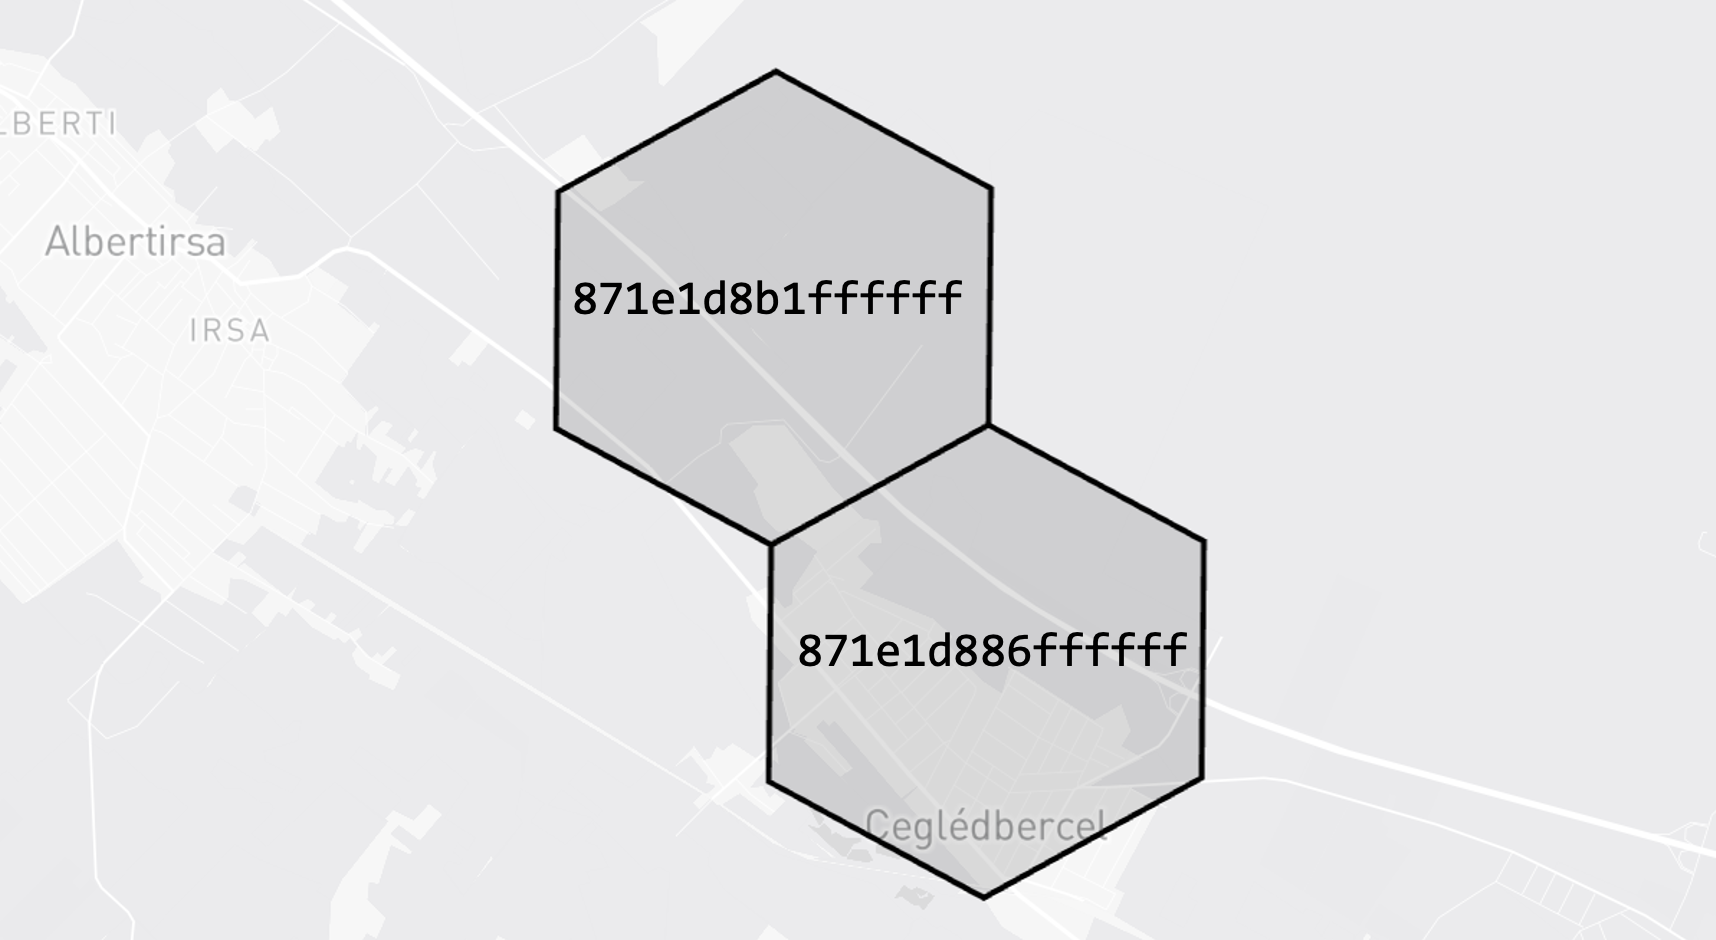
\includegraphics[width=0.7\textwidth]{images/inputdata/h3cells}
  \caption{The two H3 cells covering the captured highway section.}
  \label{fig:h3cells}
\end{figure}

Each cell contains approximately 100 million points. The intensity values range from~0 to~255, where~255 corresponds to the highest reflectivity. In cell \texttt{871e1d886ffffff}, the difference between the minimum and maximum GPS timestamp values is approximately $235\,\mathrm{s}$, indicating that the Mobile Mapping (MoMa) session traversed the highway section (in both directions) in slightly more than three minutes (see Figure~\ref{fig:cegl2gpstime}).

\begin{figure}[htbp]
  \centering
  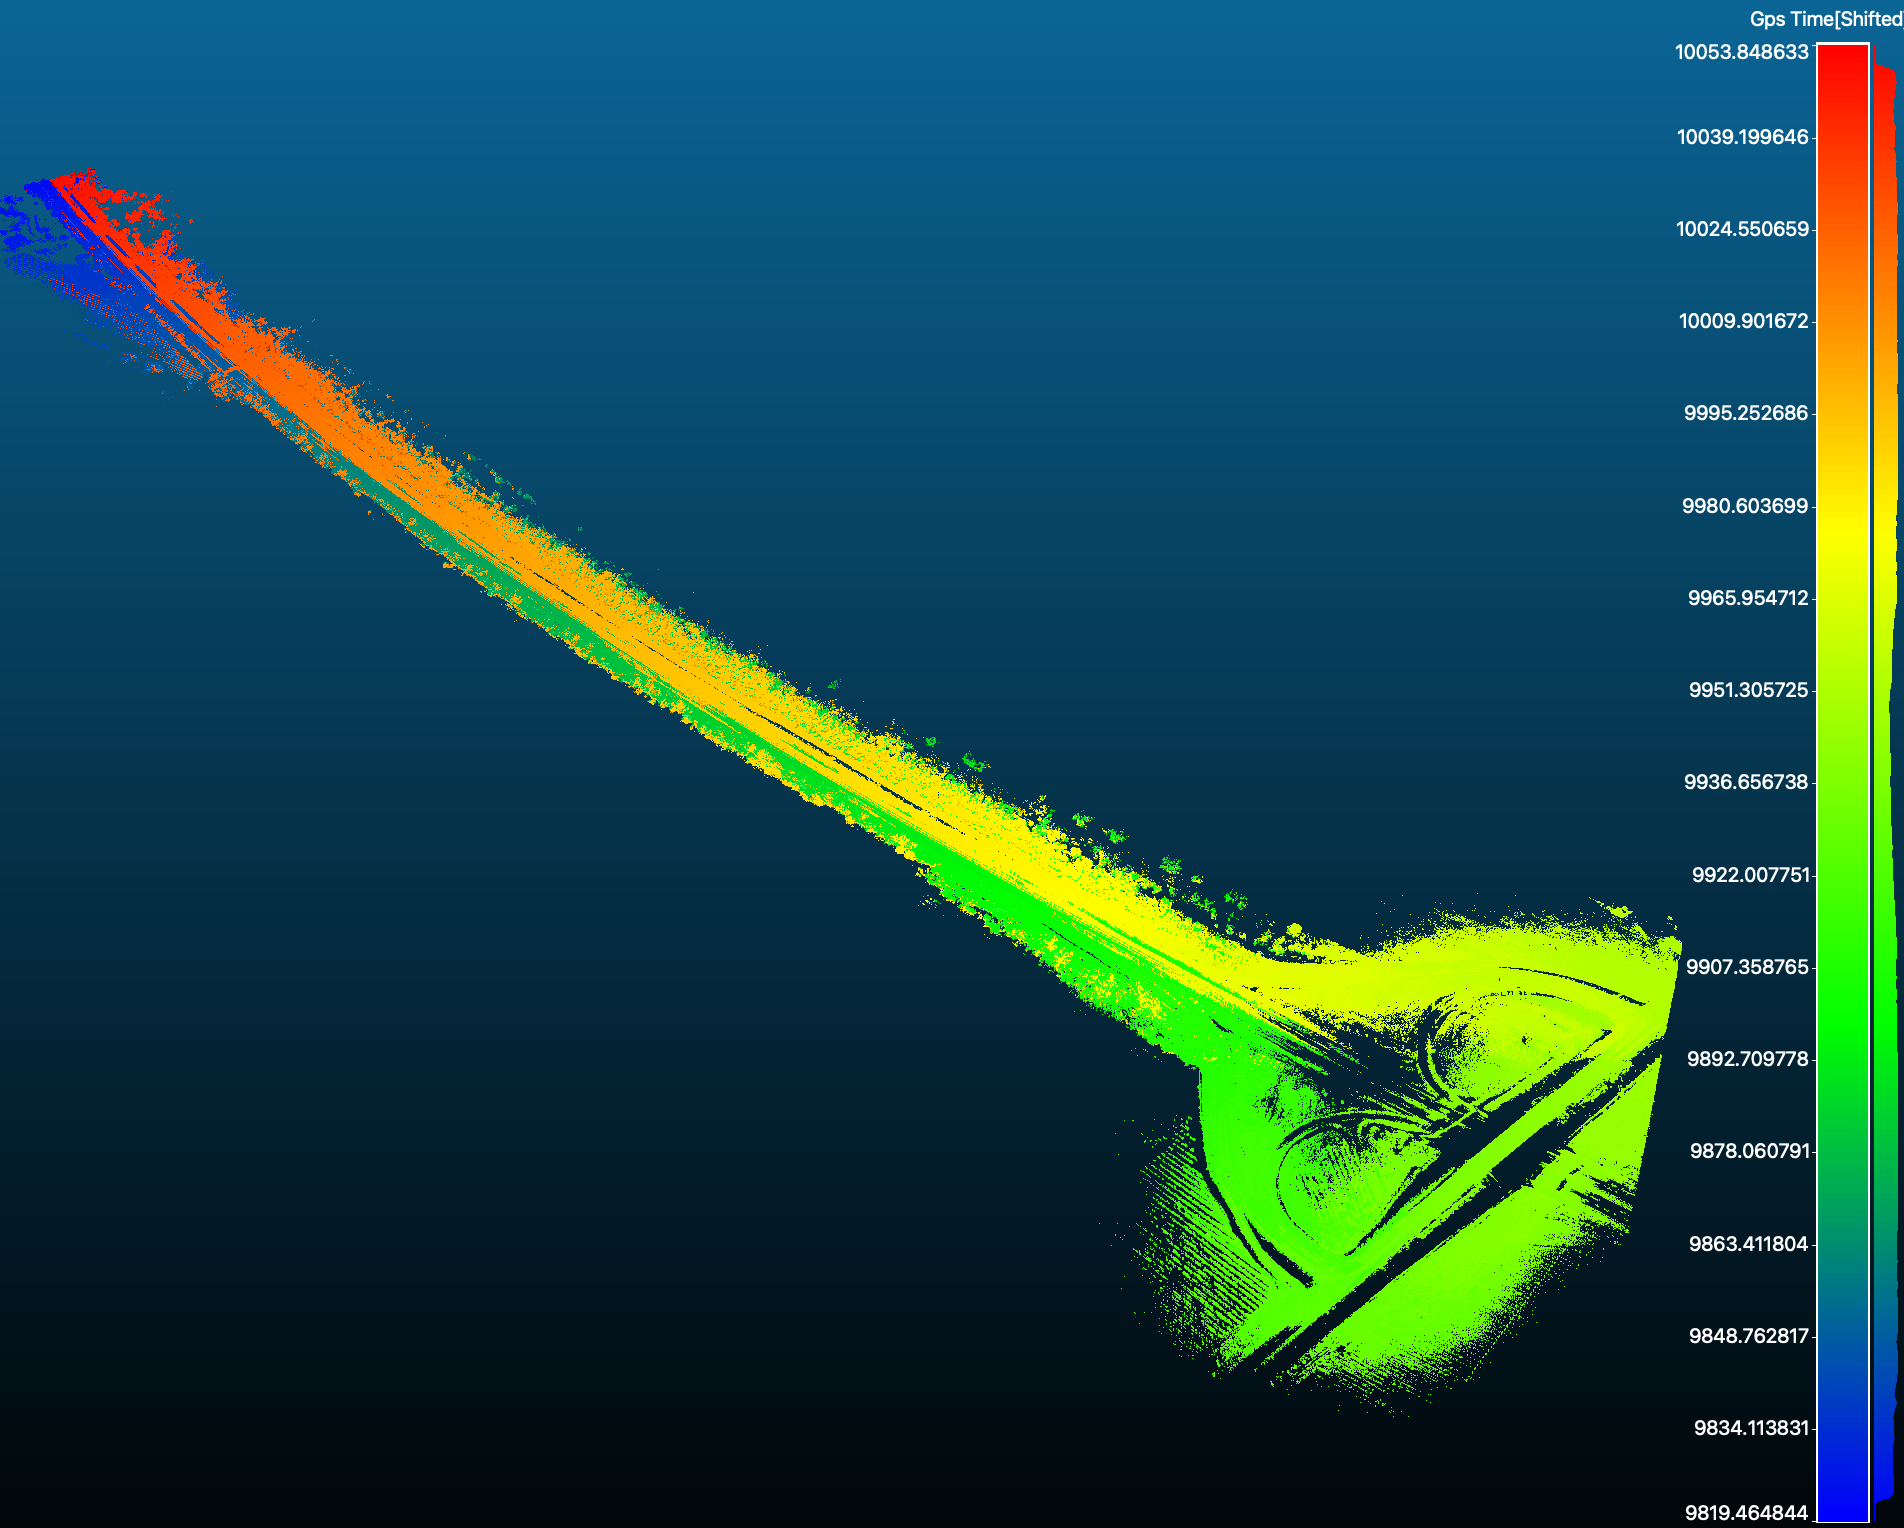
\includegraphics[width=0.7\textwidth]{images/inputdata/cegl2bytime}
  \caption{LiDAR data of cell \texttt{871e1d886ffffff} colored by GPS timestamp.}
  \label{fig:cegl2gpstime}
\end{figure}

\FloatBarrier
\subsection{Sensor Characteristics}
\label{sec:sensor}

The point cloud was captured using a Velodyne HDL-32E LiDAR sensor featuring 32 vertically stacked laser channels. During each firing sequence, the sensor emits one pulse per laser beam, yielding 32 distance measurements. A complete 32-laser firing sequence is generated every $46\,\mu\mathrm{s}$, corresponding to an effective firing frequency of approximately $21.7\,\mathrm{kHz}$.

Every 24 consecutive firing sequences are grouped into a single UDP packet, and all points within a packet share the same GPS timestamp. Consequently, each packet contains
\begin{equation}
  N_{\text{packet}} = 24 \times 32 = 768 \text{ measured points.}
  \label{eq:packet_size}
\end{equation}
\noindent In practice, fewer points are recorded because some emitted laser beams do not produce a valid return signal. Based on these values, the packet rate is approximately $900$~packets per second.

The laser channels rotate around a vertical axis at $20\,\mathrm{Hz}$, meaning that one full revolution takes $0.05\,\mathrm{s}$. Consequently, approximately 45~packets are generated during a single revolution, and each packet corresponds to roughly an $8^{\circ}$ azimuth sector of the environment, as illustrated in Figure~\ref{fig:lidarpackets}.

\begin{figure}[htbp]
  \centering
  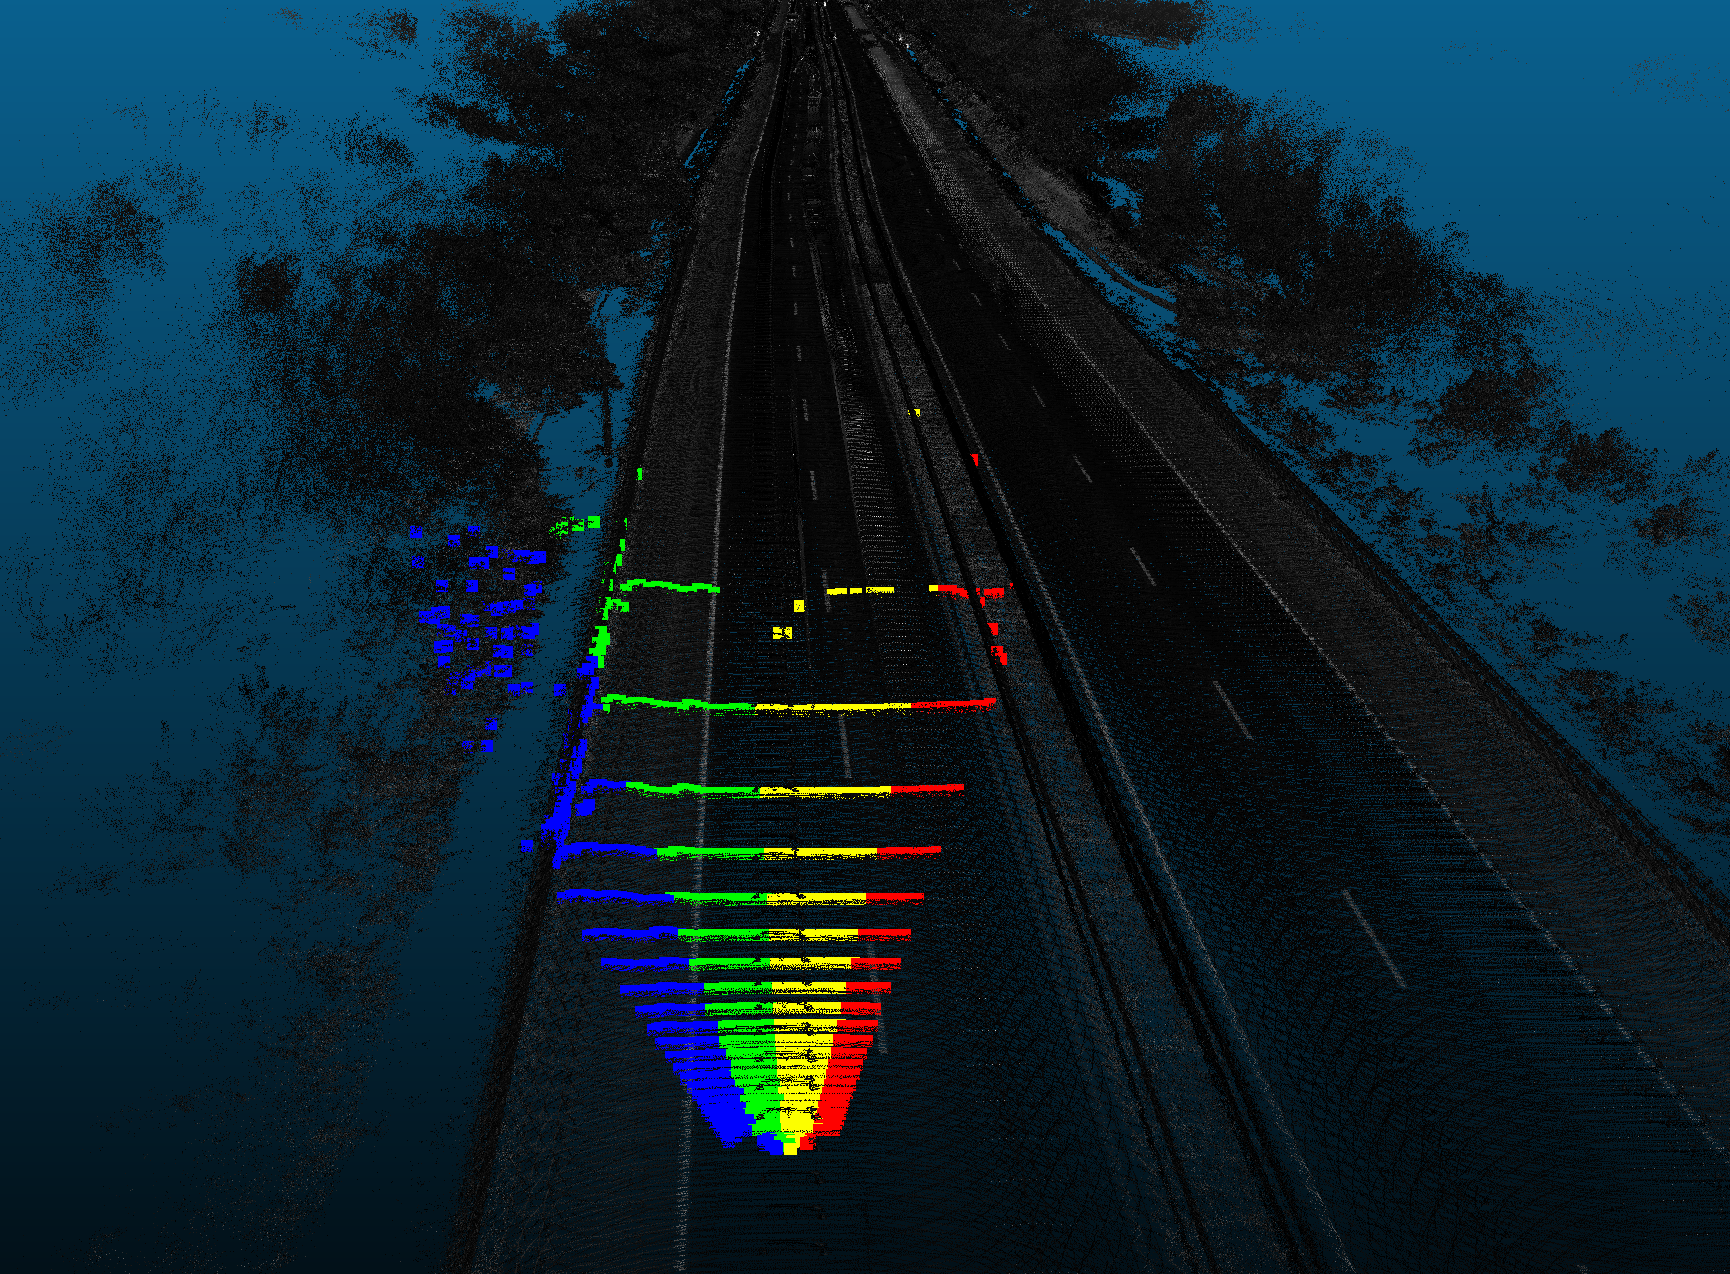
\includegraphics[width=0.7\textwidth]{images/inputdata/lidarpackets}
  \caption{A portion of the point cloud colored by intensity, with individual packets highlighted by their GPS timestamps.}
  \label{fig:lidarpackets}
\end{figure}

\FloatBarrier
\subsection{Data Structure}
\label{sec:datastructure}

By their nature, point clouds are unorganized data that require structured processing before they can be used for autonomous driving applications or, in this case, ground truth generation for road cross-sections. Table~\ref{tab:pointcloud_sample} shows a representative sample of the input data.

\begin{table}[htbp]
  \centering
  \caption{Sample records from the input point cloud.}
  \label{tab:pointcloud_sample}
  \begin{tabular}{rrrrr}
    \hline
    $x$ & $y$ & $z$ & Intensity & Timestamp \\
    \hline
    2192262.82 & 5978199.32 & 159.39 & 3  & 29922.606117 \\
    2192259.85 & 5978197.97 & 159.34 & 6  & 29922.606117 \\
    2192258.76 & 5978197.48 & 159.32 & 6  & 29922.606117 \\
    2192257.82 & 5978197.05 & 159.31 & 3  & 29922.606117 \\
    2192257.06 & 5978196.70 & 159.29 & 0  & 29922.606117 \\
    2192256.34 & 5978196.38 & 159.28 & 1  & 29922.606117 \\
    2192255.78 & 5978196.11 & 159.26 & 2  & 29922.606117 \\
    2192255.20 & 5978195.86 & 159.26 & 41 & 29922.606117 \\
    \hline
  \end{tabular}
\end{table}

\FloatBarrier
\subsection{Expected Output}
\label{sec:expected_output}

The expected output is a vectorized representation of the lane marking geometries along the recorded highway section. This representation is intended for generating ground truth cross-sections. Each geometry must be labeled according to its type: \emph{solid} or \emph{dashed}. The pipeline produces a GeoPackage file containing multiple LineString geometries, each annotated with a \texttt{type} attribute set to either \texttt{solid} or \texttt{dashed}.

%------------------------------------------------------------------
\section{Pipeline Overview}
\label{sec:pipeline_overview}

The pipeline consists of multiple interdependent processing stages organized into three major phases (see Figure~\ref{fig:process}):

\begin{enumerate}
  \item \textbf{Vehicle trajectory reconstruction} (Section~\ref{sec:car_trace}):
  \begin{enumerate}
    \item Reconstruct the vehicle trajectory from LiDAR timestamps, providing an initial estimate of the lane positions.
  \end{enumerate}

  \item \textbf{Point cloud processing} (Section~\ref{sec:pointcloud_processing}):
  \begin{enumerate}
    \item Bin the point cloud along the vehicle trace and process it in overlapping windows.
    \item Remove distant points using trace-based clipping.
    \item Segment ground and non-ground points using RANSAC-based plane detection~\cite{RANSAC}.
    \item Detect the road surface using region-growing methods seeded from the trace.
    \item Segment road markings using intensity thresholding (Kapur maximum-entropy method~\cite{KAPUR1985273} or percentile-based thresholding).
  \end{enumerate}

  \item \textbf{Line fitting on road markings} (Section~\ref{sec:line_fitting}):
  \begin{enumerate}
    \item Cluster and track lane marking points across overlapping windows.
    \item Fit and refine vectorized lane curves using constrained quadratic RANSAC and moving least squares.
    \item Label lane types (solid or dashed) based on point continuity.
  \end{enumerate}
\end{enumerate}

\noindent Finally, the detected lanes are exported as georeferenced vector representations.

\begin{figure}[htbp]
  \centering
  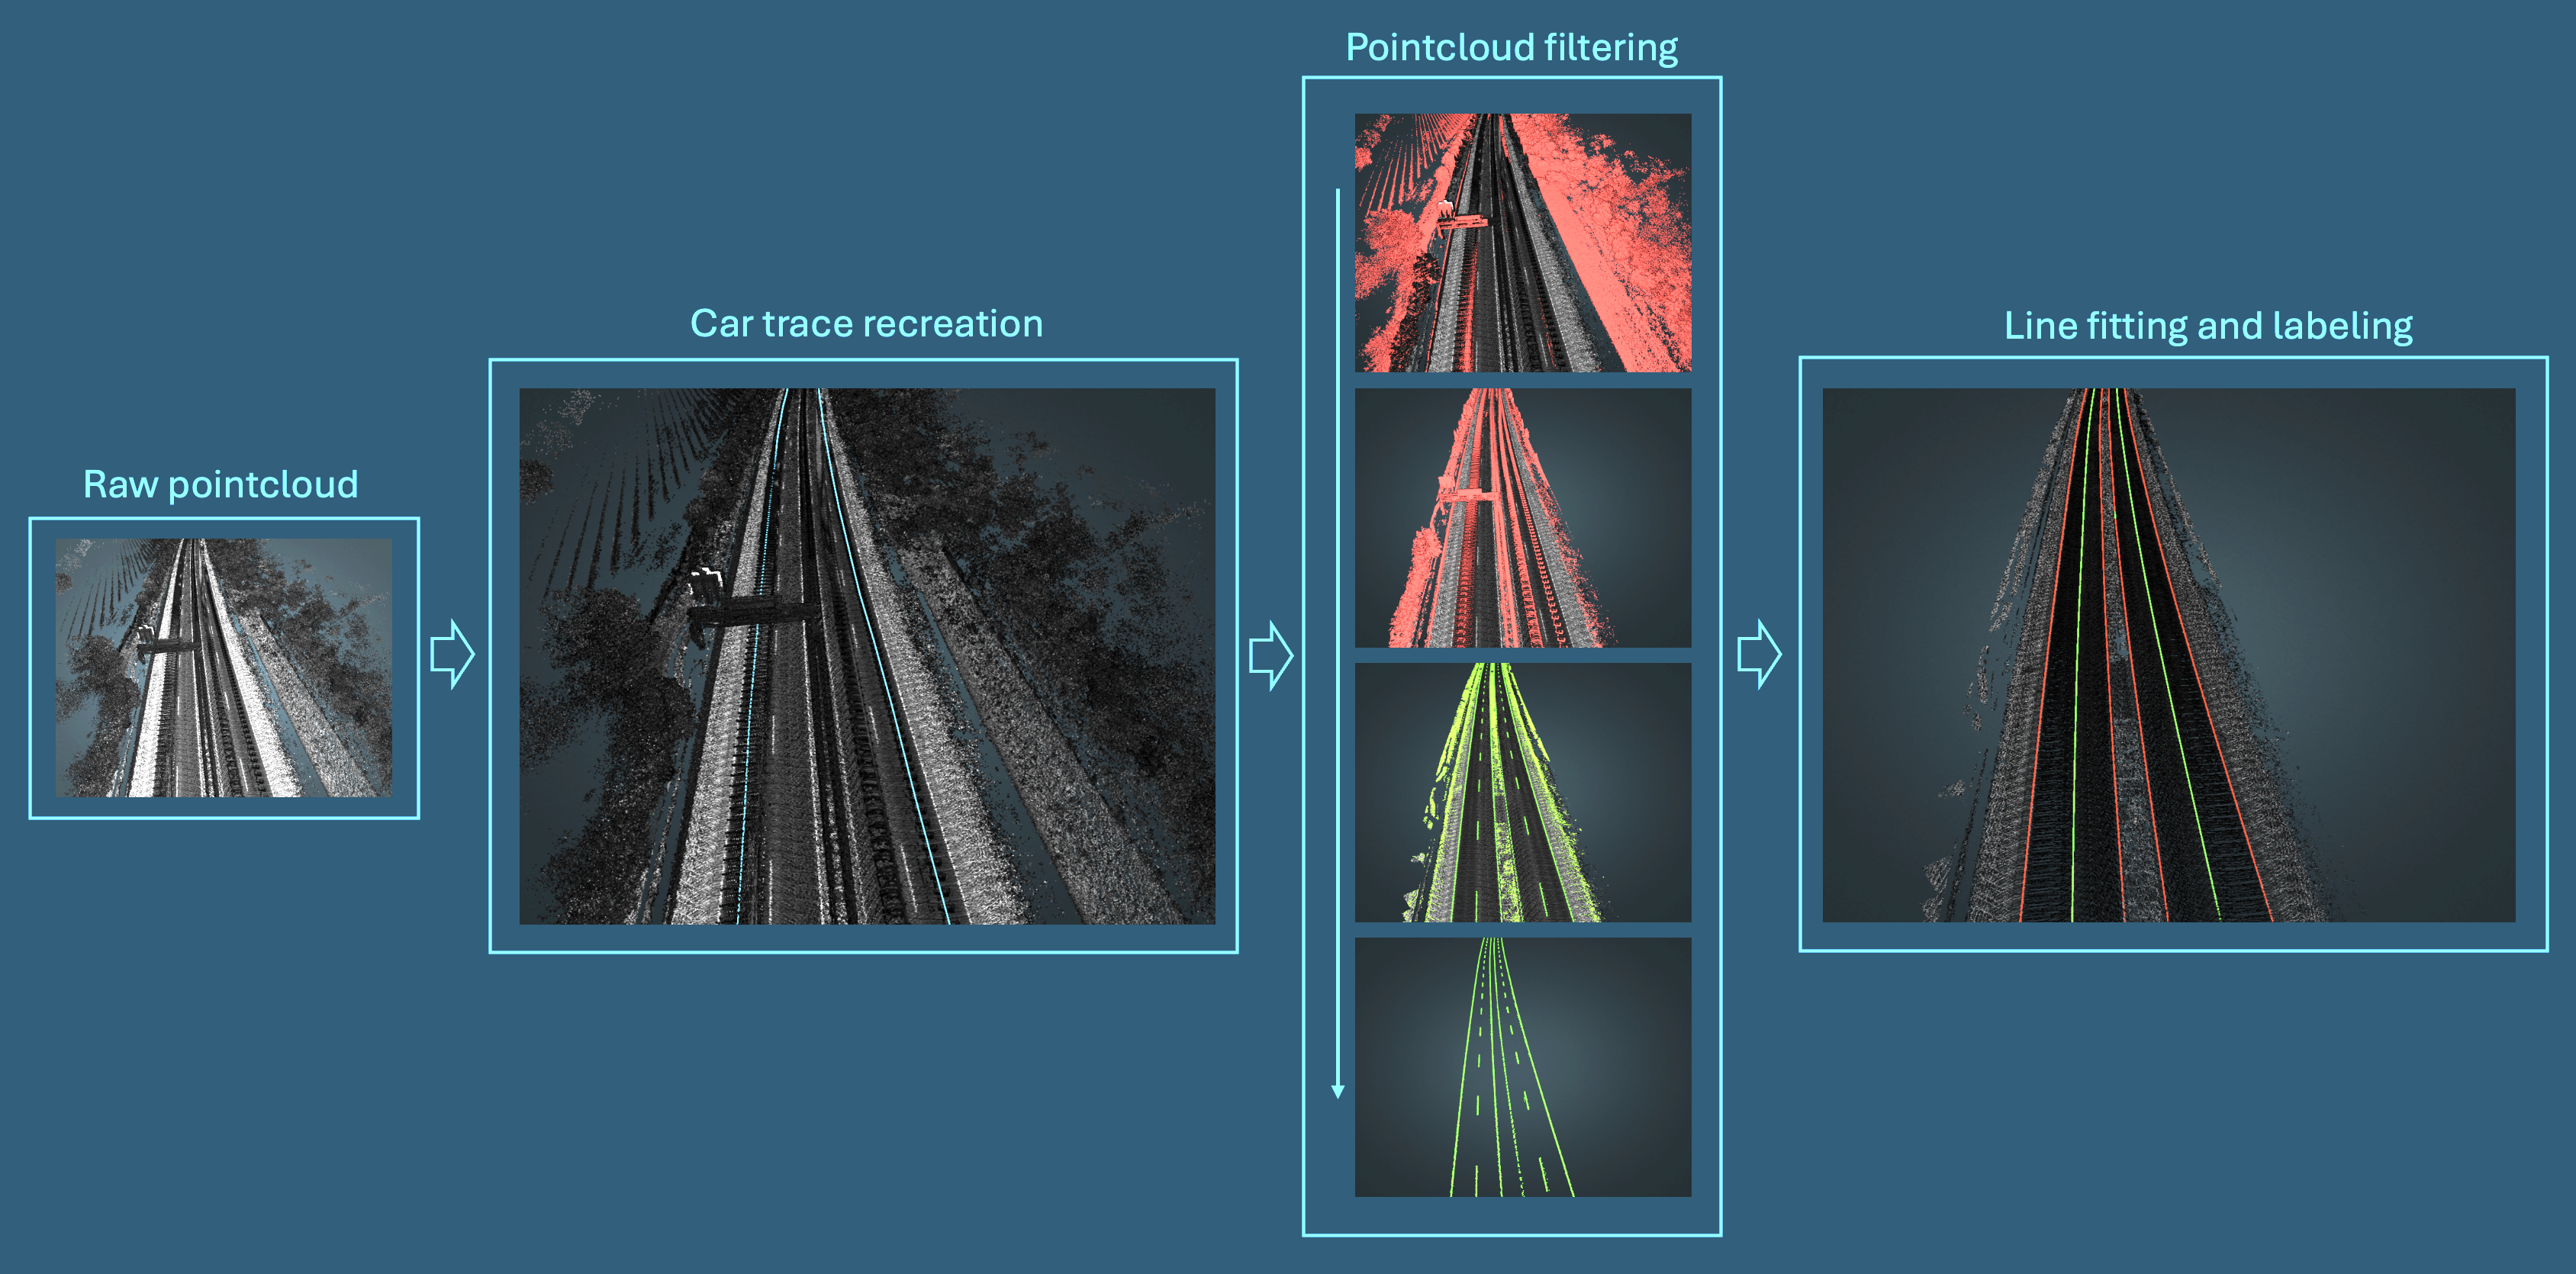
\includegraphics[width=0.9\textwidth]{images/process}
  \caption{High-level overview of the lane detection pipeline, showing the three major phases: trajectory reconstruction, point cloud processing, and line fitting.}
  \label{fig:process}
\end{figure}

%------------------------------------------------------------------
\section{Vehicle Trajectory Reconstruction}
\label{sec:car_trace}

Knowledge of the mapping vehicle's trajectory is essential for the pipeline. Given the trajectory, an initial estimate of the lane positions can be derived, since the vehicle is assumed to have traveled within a lane throughout the recording session. However, since no trajectory data was provided with the dataset, it must be recovered from the properties of the point cloud itself.

The following assumptions are made:
\begin{itemize}
  \item The MoMa vehicle traveled exclusively on the road surface.
  \item The LiDAR sensor was mounted on the vehicle.
  \item The computed trajectory should lie on the road surface, as this property is exploited in subsequent processing stages.
\end{itemize}

\noindent Only the $xy$-coordinates of the trajectory are required; the elevation component is disregarded. Each algorithm effectively estimates the position of the LiDAR sensor, which is assumed to coincide with the vehicle position.

To evaluate the trajectory reconstruction algorithms, a ground truth trajectory spanning $4700\,\mathrm{m}$ was manually annotated. This was feasible because the LiDAR sensor captured a small portion of the vehicle's trunk during every revolution (visible in Figure~\ref{fig:window_median_result}). The quantitative evaluation of the algorithms is presented in Chapter~\ref{ch:eval}.

Four algorithms were developed: a simple baseline method followed by three progressively more sophisticated approaches. The pipeline defaults to the Pulse Line algorithm (Section~\ref{sec:pulse_lines}), which yielded the most accurate trajectory estimates.

\FloatBarrier
\subsection{Window Median (Baseline)}
\label{sec:window_median}

As established in Section~\ref{sec:sensor}, the LiDAR sensor completes one full revolution in approximately $0.05\,\mathrm{s}$. Under ideal conditions---where every laser beam produces a valid return and all recorded points are equidistant from the sensor---the vehicle position coincides exactly with the median of the points recorded during one revolution. This ideal scenario requires:
\begin{itemize}
  \item Every laser beam produces a valid reflection that is recorded by the sensor.
  \item In every firing sequence, the nearest point reflects off the ground surface.
  \item The sensor's rotation axis is perpendicular to the vehicle's horizontal plane.
\end{itemize}

\noindent When any of these conditions is violated, the median-based estimate can become biased. Figure~\ref{fig:window_median_illustration} illustrates this phenomenon: in practice, roadside objects (e.g., trees) on one side reflect more laser beams than the open space on the other side, causing the median to shift away from the true sensor position.


\begin{figure}[htbp]
  \centering
  \begin{subfigure}[b]{0.48\textwidth}
    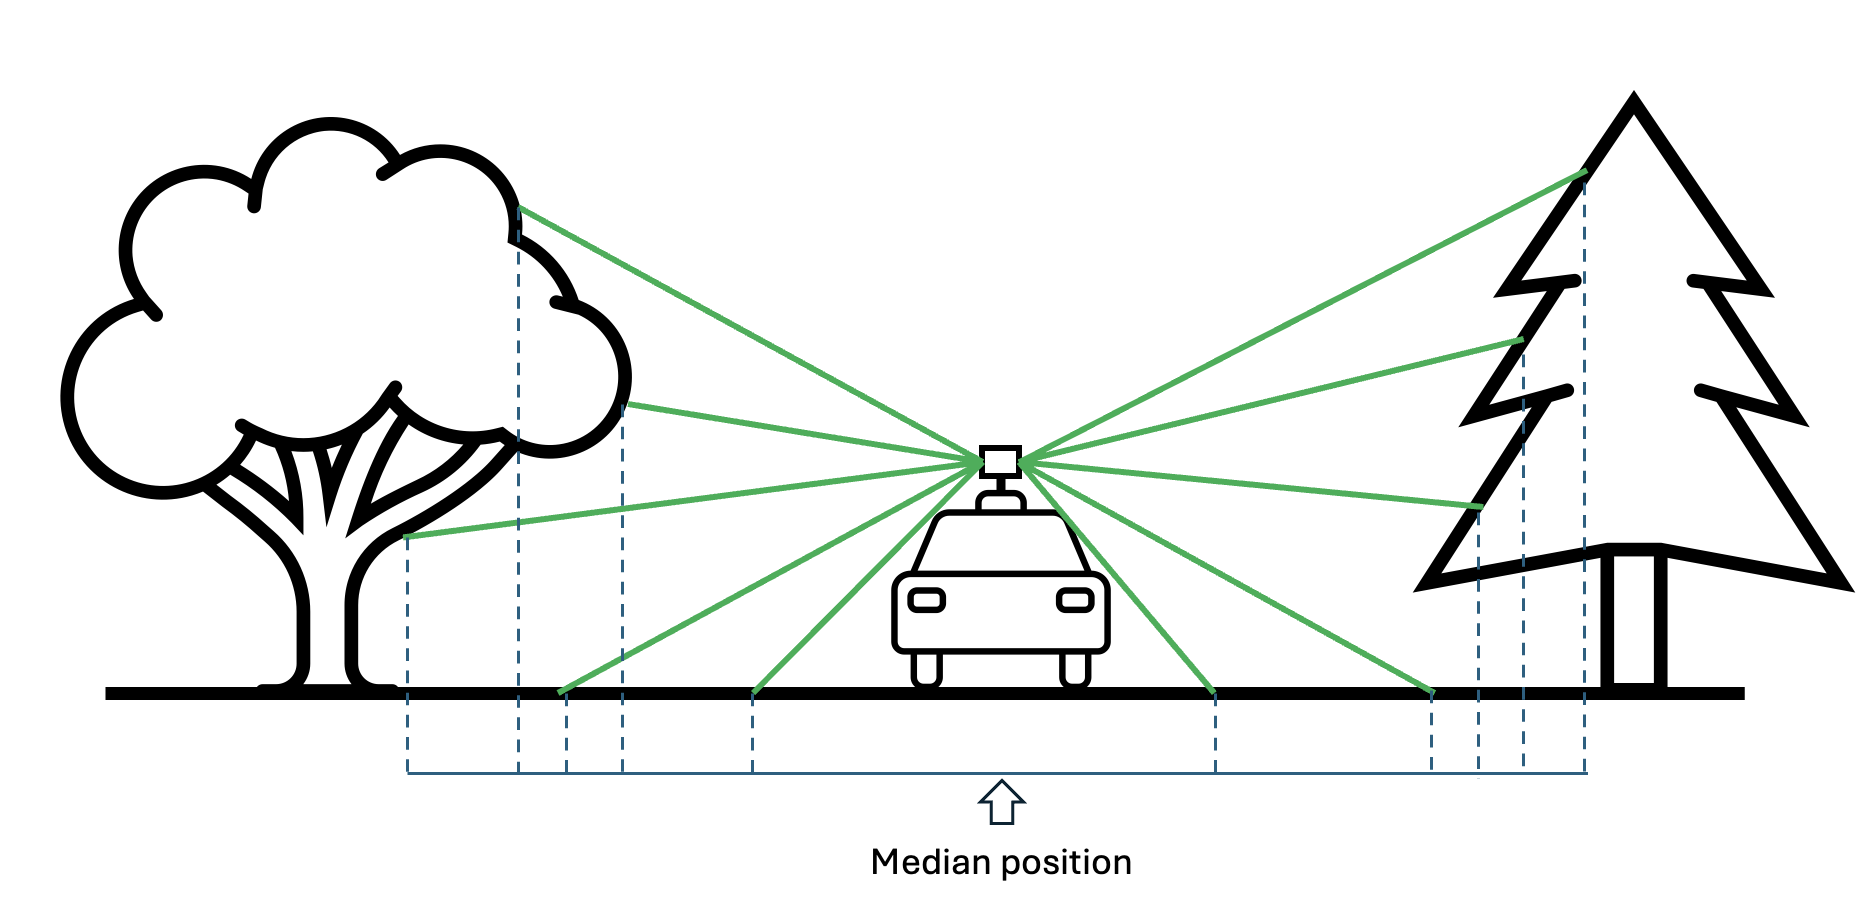
\includegraphics[width=\textwidth]{images/car_trace/window_median_illutstration}
    \caption{Visualization of the ideal situation.}
  \end{subfigure}
  \hfill
  \begin{subfigure}[b]{0.48\textwidth}
    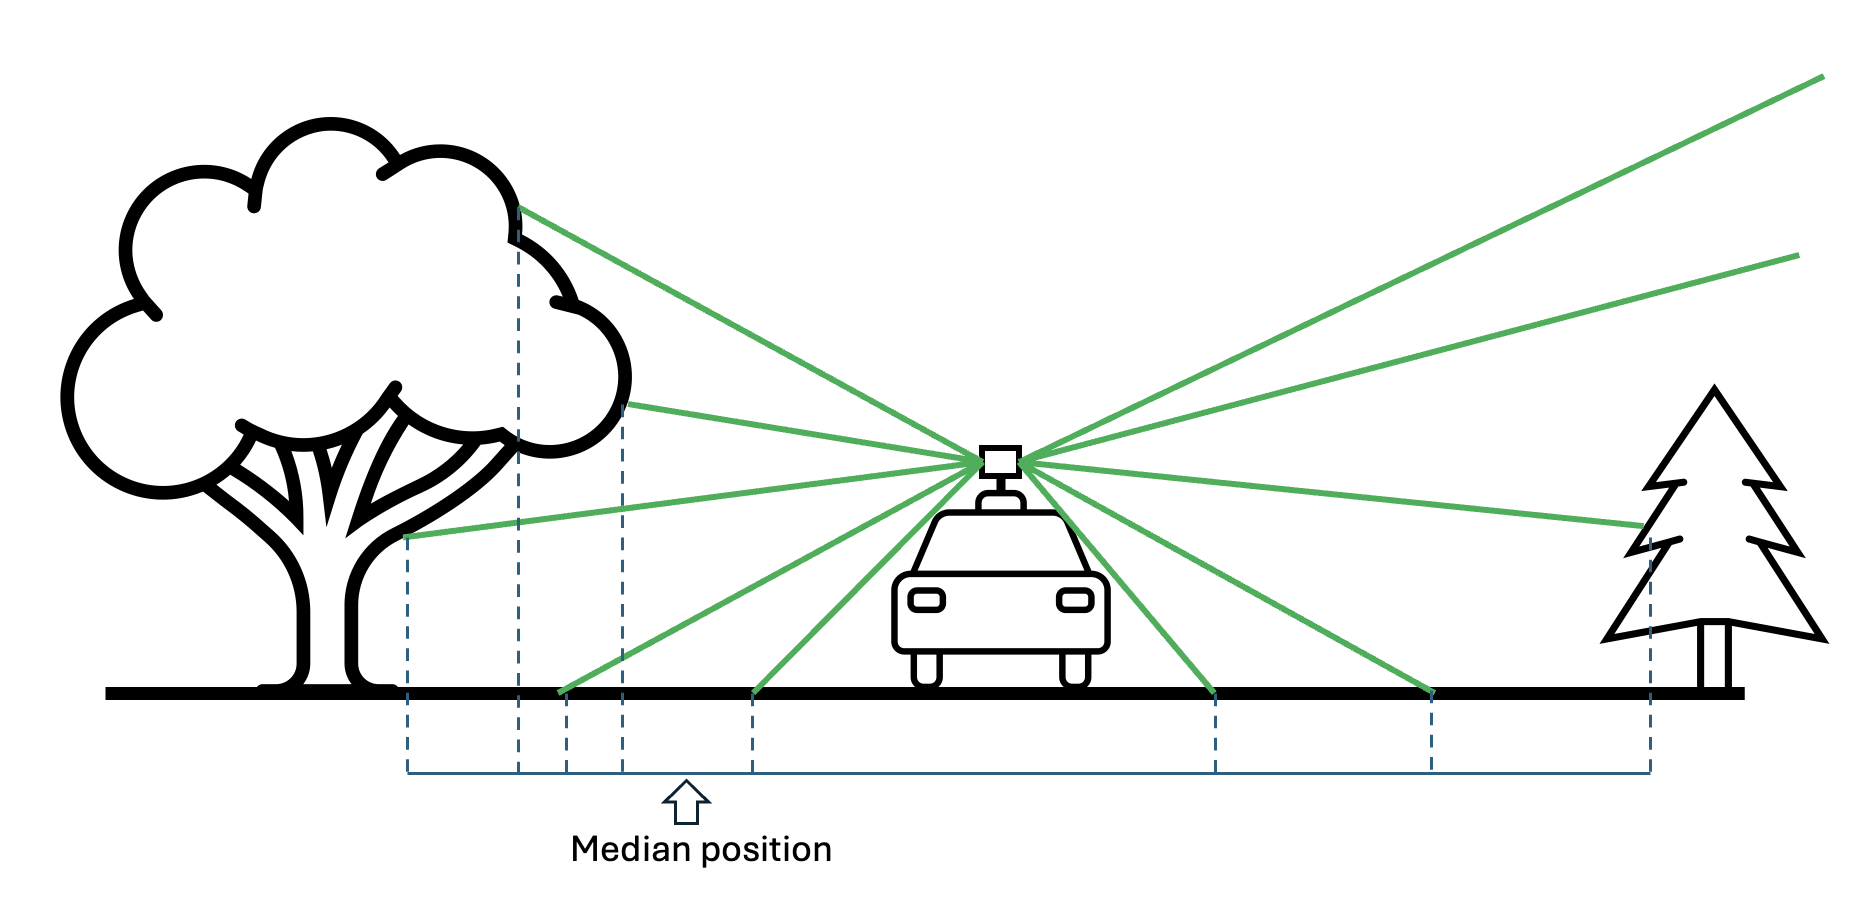
\includegraphics[width=\textwidth]{images/car_trace/window_median_illutstration_real}
    \caption{Uneven number of reflections.}
  \end{subfigure}
  \caption{Illustration of the Window Median algorithm, and it's defect: (a)~In the ideal situation both sides have the same amount of reflected points (b)~in typical scenarios, one side has more reflection.}
  \label{fig:window_median_illustration}
\end{figure}

The algorithm proceeds as follows:
\begin{enumerate}
  \item Select a temporal window of scanned points at regular time intervals.
  \item Compute the median of the $xy$-coordinates of all points within the window as the estimated vehicle position.
  \item Append the estimated positions sequentially to form a LineString geometry.
  \item Export the result to a GeoPackage file for subsequent evaluation.
\end{enumerate}

Despite its simplicity, this baseline method provides a surprisingly accurate approximation in the majority of cases. However, as shown in Figure~\ref{fig:window_median_result}, the estimate exhibits a systematic lateral bias: trees on the right side of the vehicle reflect more laser beams than the open left side, pulling the median toward the right.

\begin{figure}[htbp]
  \centering
  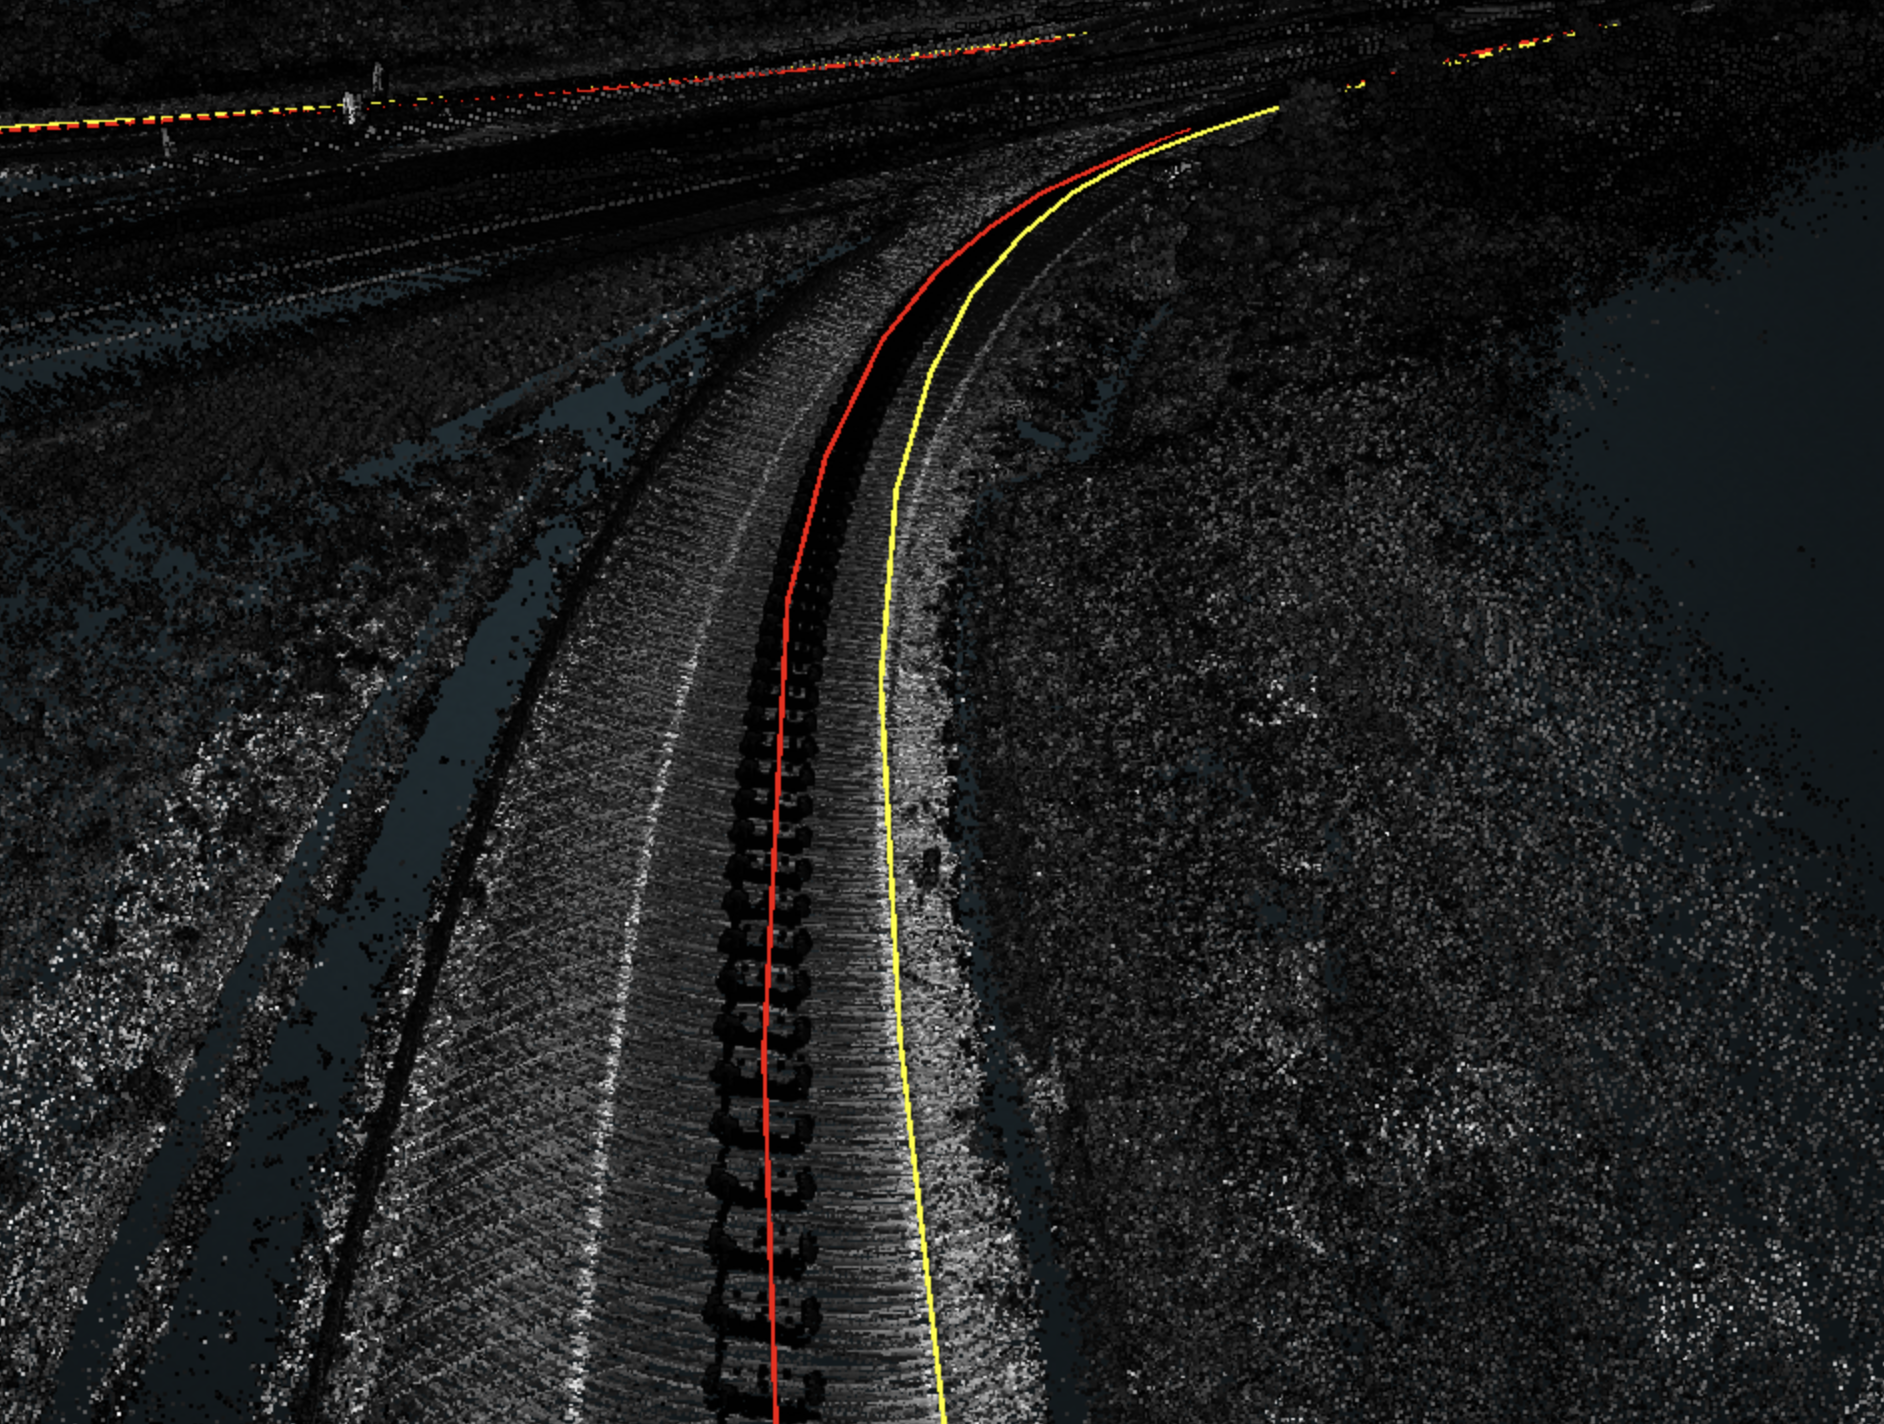
\includegraphics[width=0.7\textwidth]{images/car_trace/window_median_result}
  \caption{Comparison of the ground truth trajectory (red) and the Window Median baseline estimate (yellow). The systematic rightward bias is caused by asymmetric reflections from roadside vegetation.}
  \label{fig:window_median_result}
\end{figure}

\FloatBarrier
\subsection{Window Median with Ground Filtering}
\label{sec:window_median_v2}

This algorithm addresses the primary weakness of the baseline method. The key insight is that if points above a certain height threshold could be identified and excluded---particularly those reflected from elevated objects that are not symmetrically distributed---the resulting median would be significantly less biased. This approach assumes that downward-directed laser beams consistently produce valid ground returns.

The algorithm operates as follows:
\begin{enumerate}
  \item At regular time intervals, select a temporal window of points.
  \item Compute the median of the $xy$-coordinates as an initial position estimate.
  \item At the estimated position, determine the ground plane using iterative RANSAC-based plane fitting.
  \item Discard all points whose elevation exceeds the ground level by more than a specified offset $\Delta z$.
  \item Recompute the median of the remaining points as the refined vehicle position estimate.
\end{enumerate}

\begin{figure}[htbp]
  \centering
  \begin{subfigure}[b]{0.7\textwidth}
    \centering
    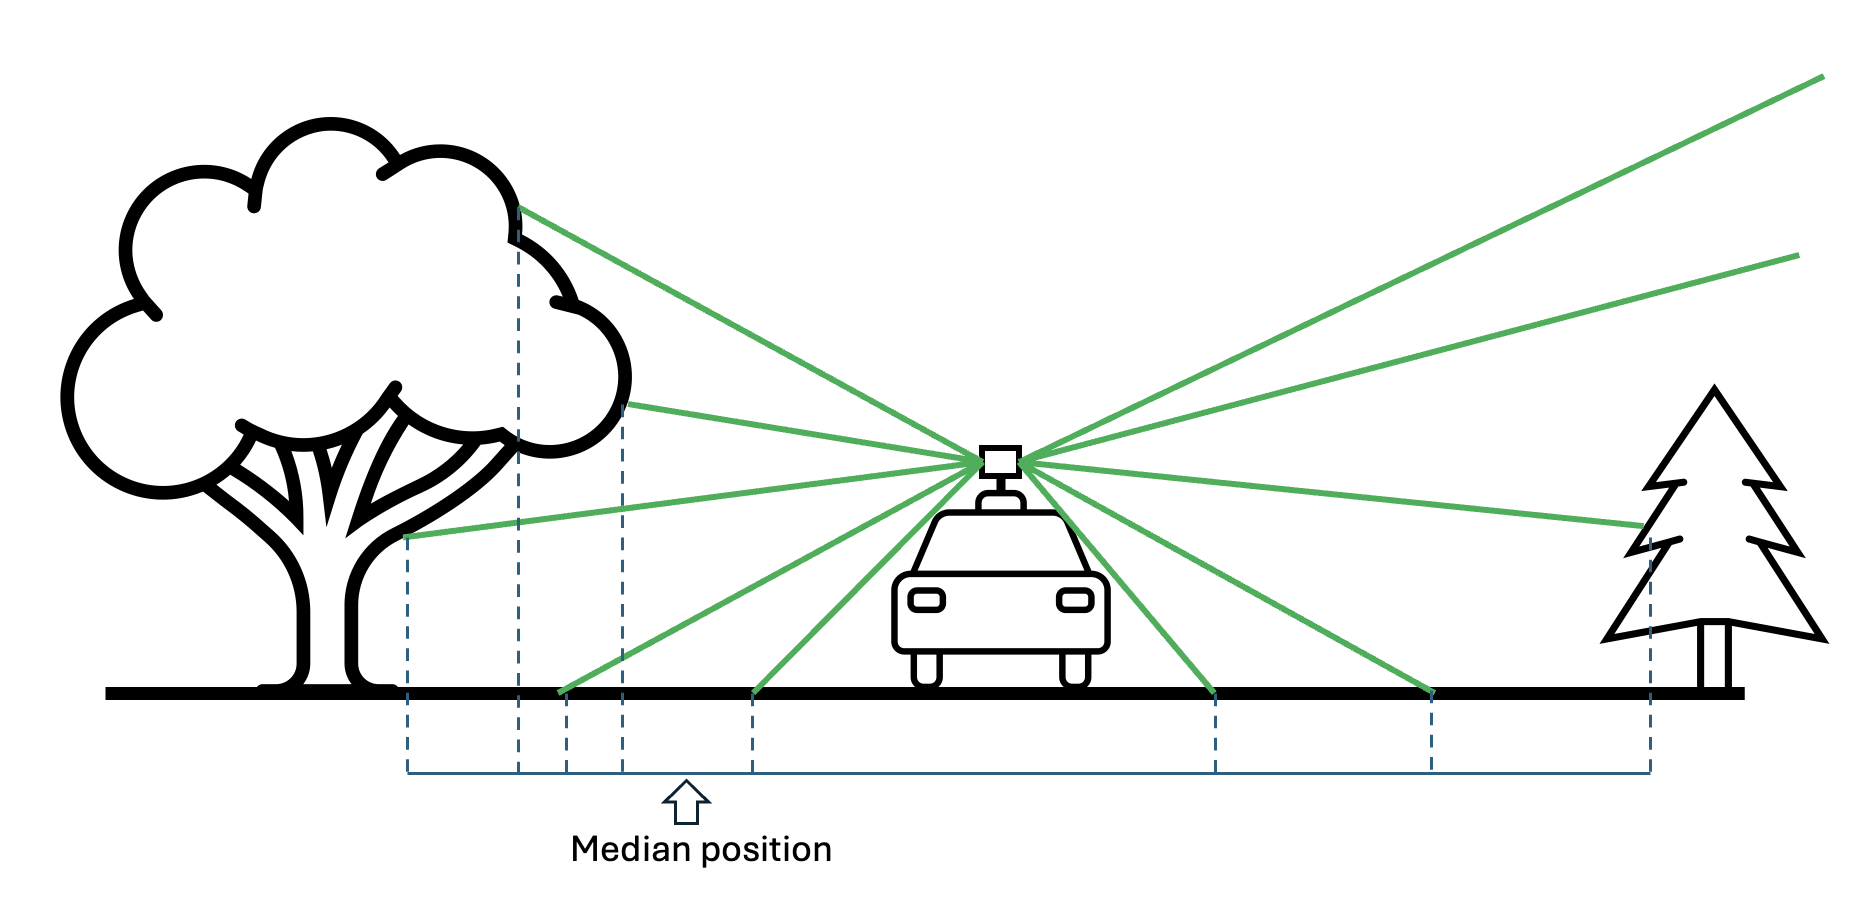
\includegraphics[width=\textwidth]{images/car_trace/window_median_illutstration_real}
    \caption{Biased baseline estimate.}
    \label{fig:wm_v2_bias}
  \end{subfigure}
  \\[0.5em]
  \begin{subfigure}[b]{0.7\textwidth}
    \centering
    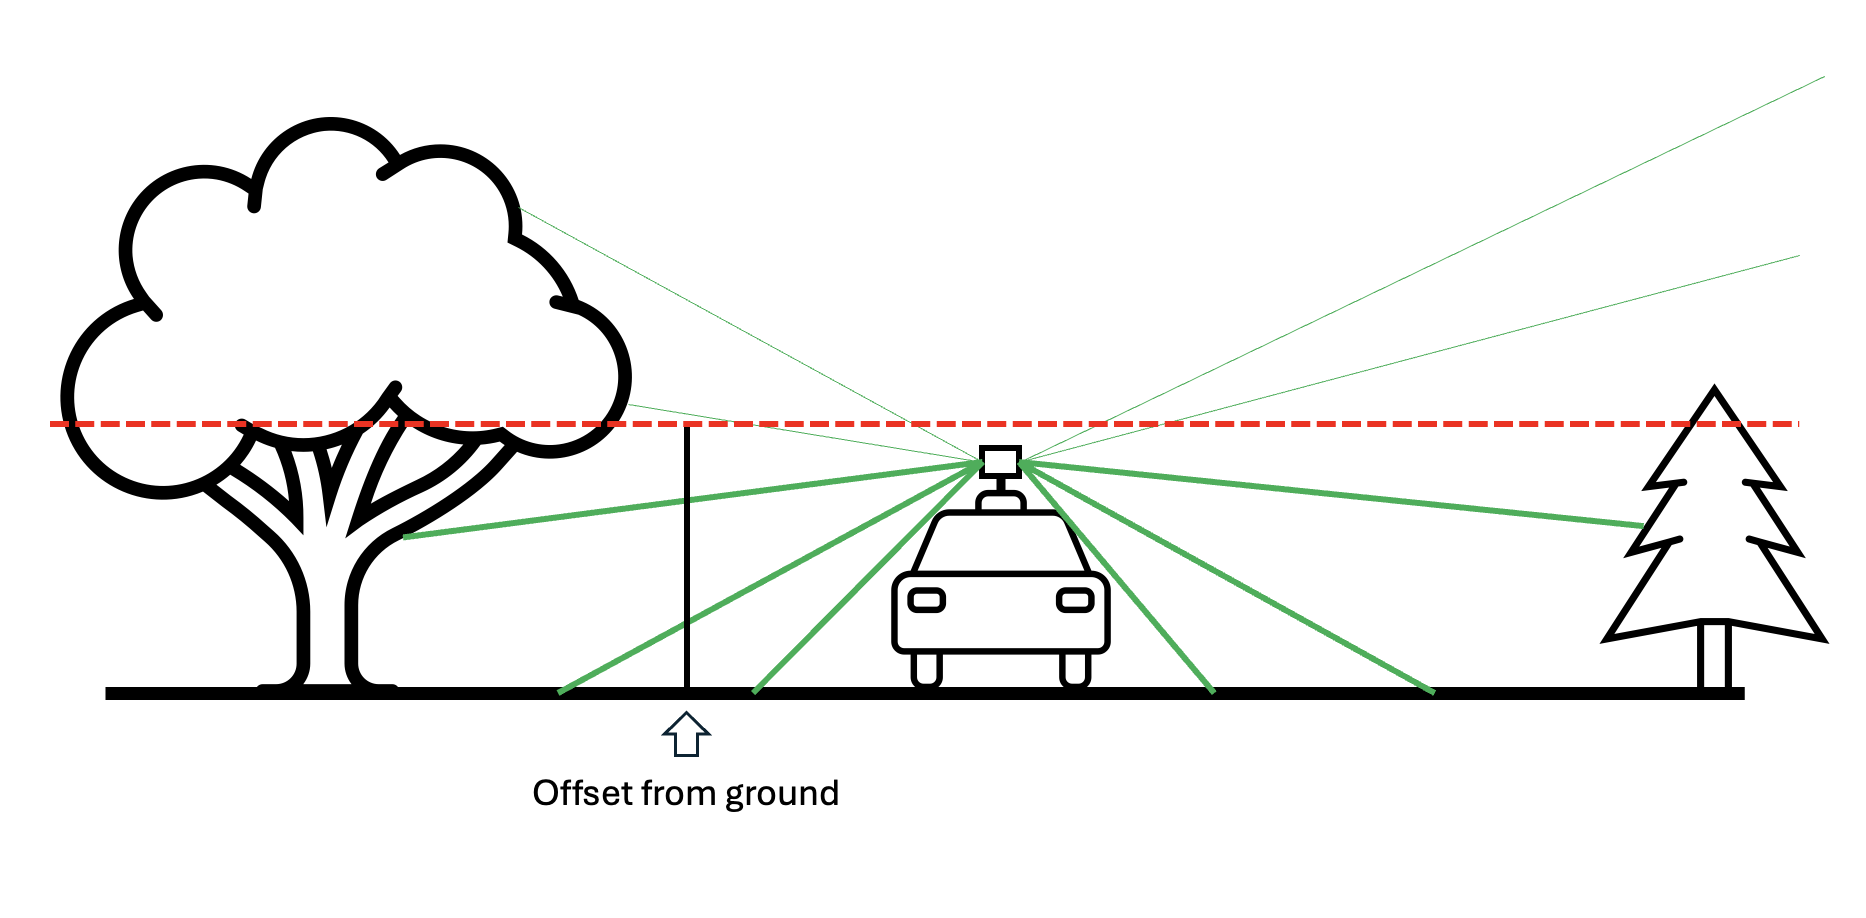
\includegraphics[width=\textwidth]{images/car_trace/window_median_v2_offset}
    \caption{Points above ground $+ \Delta z$ are discarded.}
    \label{fig:wm_v2_offset}
  \end{subfigure}
  \\[0.5em]
  \begin{subfigure}[b]{0.7\textwidth}
    \centering
    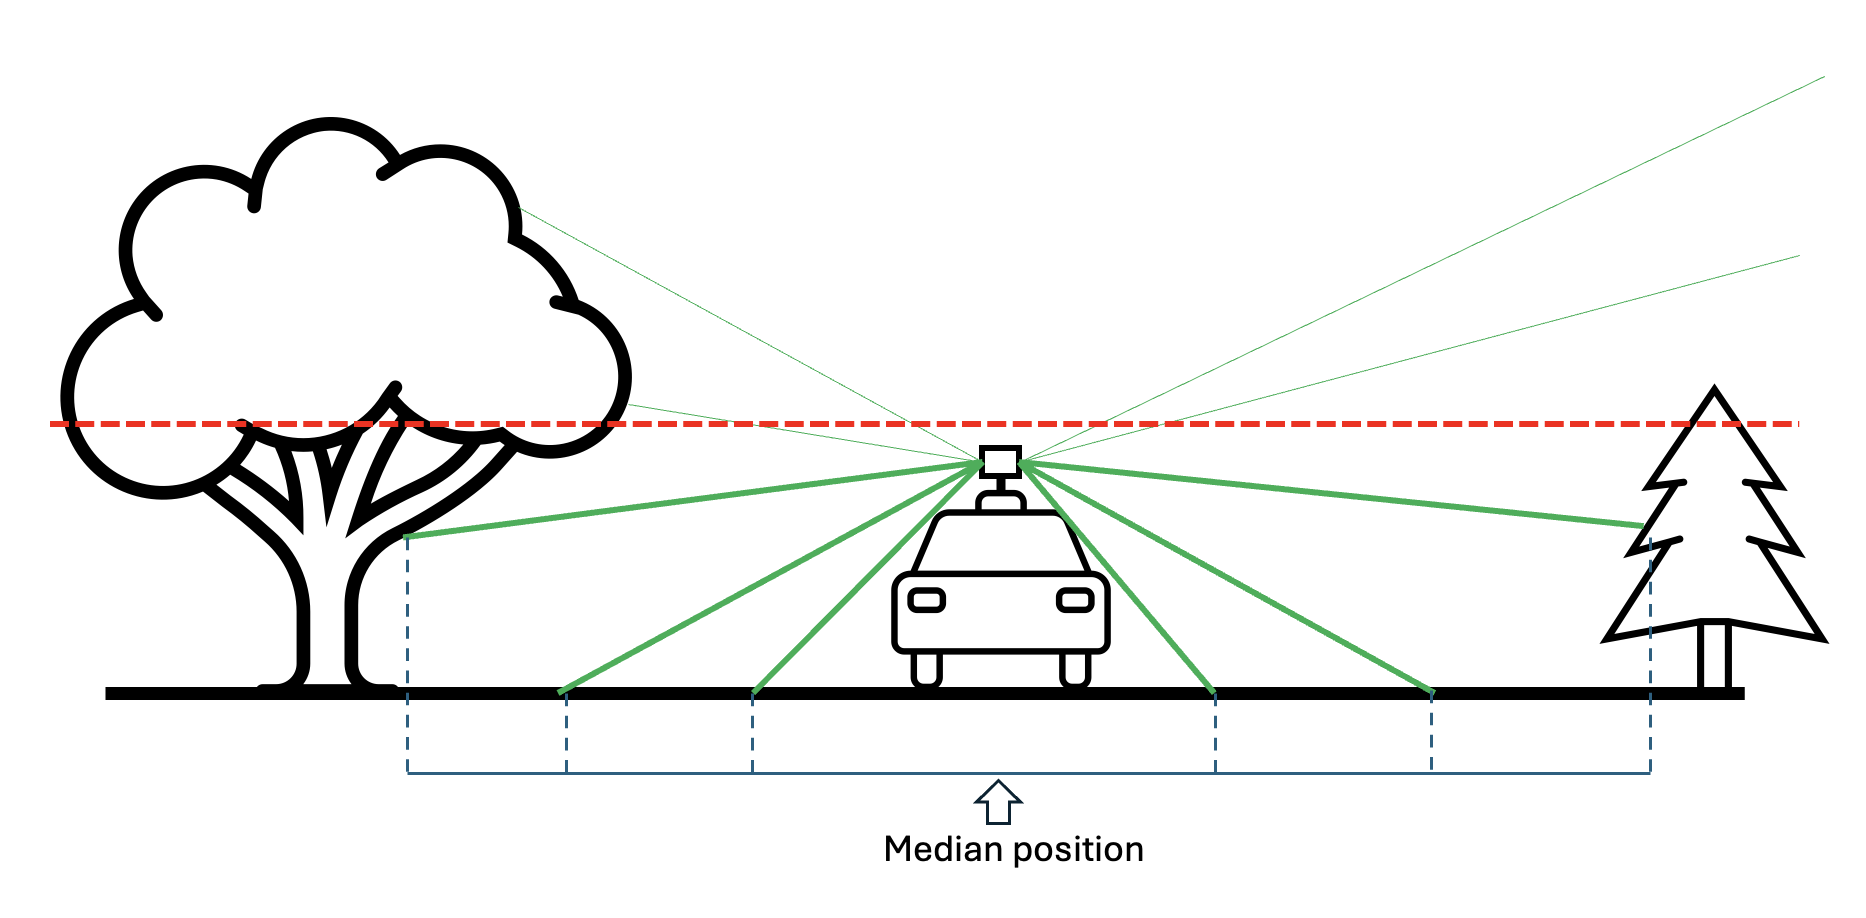
\includegraphics[width=\textwidth]{images/car_trace/window_median_v2}
    \caption{Corrected position estimate.}
    \label{fig:wm_v2_corrected}
  \end{subfigure}
  \caption{Illustration of the Window Median with Ground Filtering algorithm: (a)~the baseline produces a biased estimate; (b)~points above the ground plane plus an offset are removed; (c)~the recomputed median yields an improved estimate.}
  \label{fig:window_median_v2_illustration}
\end{figure}

As demonstrated in Figure~\ref{fig:window_median_v2_result}, this method provides a substantial improvement over the baseline. However, it is only effective when the initial (unfiltered) median estimate is already reasonably close to the true vehicle position.

\begin{figure}[htbp]
  \centering
  \includegraphics[width=0.7\textwidth]{images/car_trace/window_median_v2_result}
  \caption{Comparison of trajectory estimates: ground truth (red), Window Median baseline (yellow), and Window Median with Ground Filtering (orange).}
  \label{fig:window_median_v2_result}
\end{figure}

\FloatBarrier
\subsection{Pulse Line Intersection}
\label{sec:pulse_lines}

This algorithm exploits a geometric property of the LiDAR sensor's packet structure. As established in Section~\ref{sec:sensor}, points sharing the same GPS timestamp occupy an approximately $8^{\circ}$ unbounded angular sector originating from the LiDAR sensor. The center of this sector---the point from which the laser beams emanate---corresponds to the sensor position.

The algorithm is as follows:
\begin{enumerate}
  \item At regular intervals, select a packet (i.e., a set of points sharing a common GPS timestamp).
  \item Fit a regression line to the $xy$-coordinates of the packet's points using ordinary least squares.
  \item Advance through subsequent packets until a packet is found whose regression line forms a sufficiently large angle with the first.
  \item Compute the intersection of the two regression lines; this intersection is taken as the estimated sensor position.
\end{enumerate}

\noindent The geometric principle is illustrated in Figure~\ref{fig:pulse_lines}: since each packet's points lie along a narrow angular sector, their regression lines converge at the sensor location.

\begin{figure}[htbp]
  \centering
  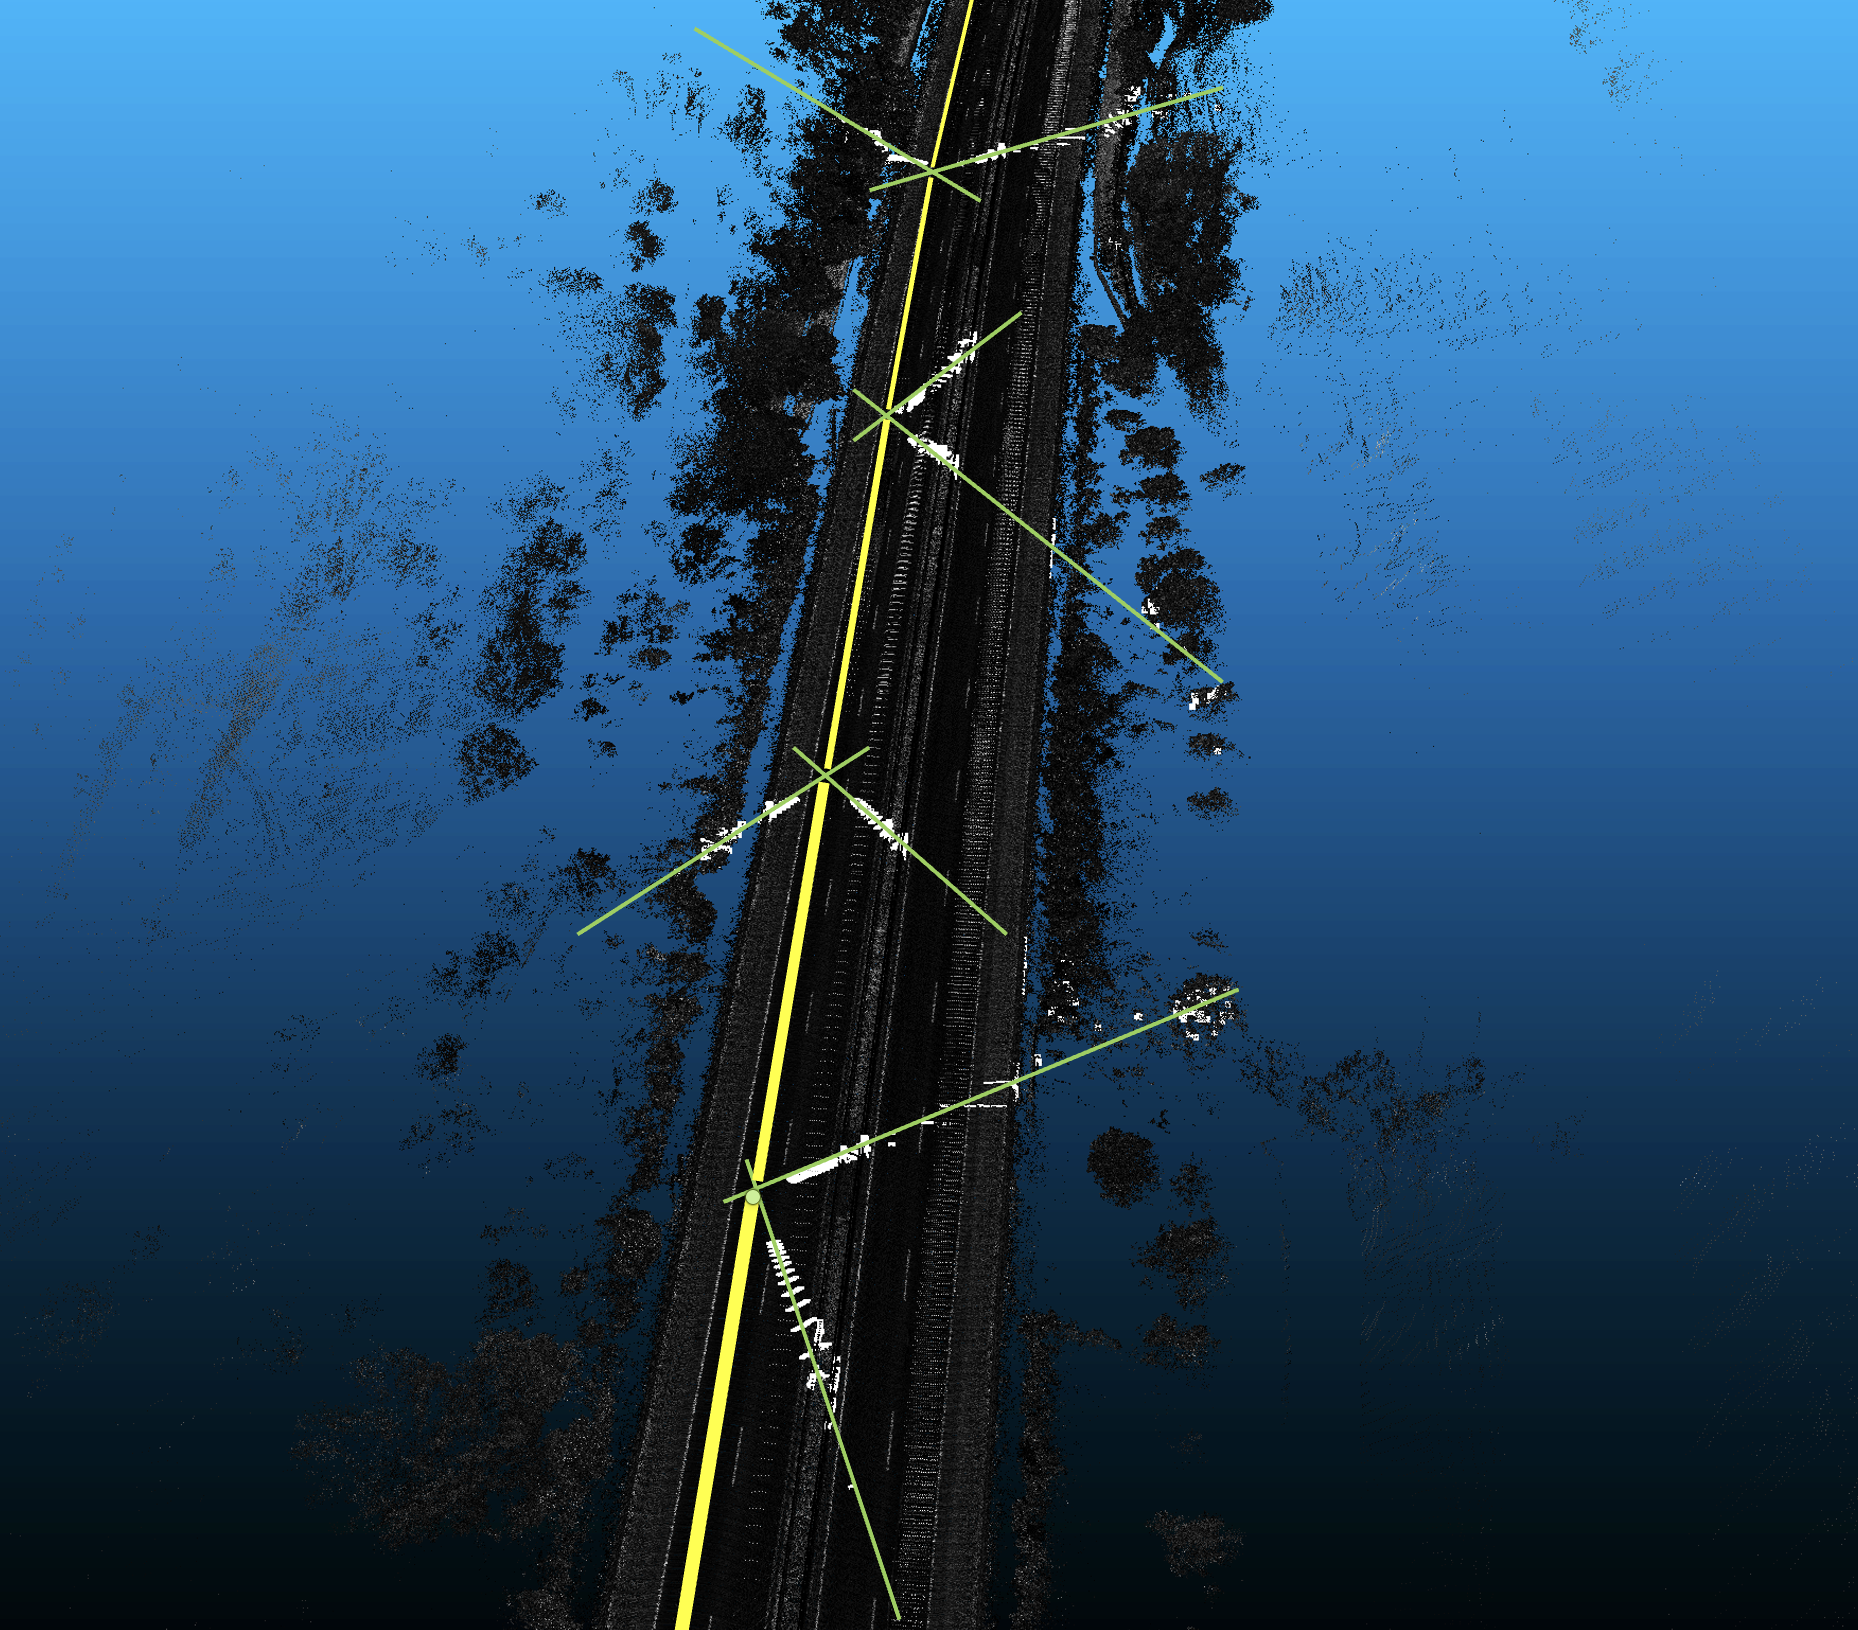
\includegraphics[width=0.7\textwidth]{images/car_trace/pulse_lines}
  \caption{The Pulse Line Intersection algorithm: regression lines fitted to individual packets intersect at the estimated sensor position.}
  \label{fig:pulse_lines}
\end{figure}

This algorithm produced highly accurate position estimates among all four methods (quantitative evaluation in Chapter~\ref{ch:eval}) and is therefore used as the default trajectory reconstruction method in the pipeline.

\FloatBarrier
\subsection{Closest Point Convergence}
\label{sec:closest_point}

This algorithm is based on the following observation: if the vehicle position is initialized at an arbitrary point and, for each successive packet, the estimate is updated to the point within that packet closest to the previous estimate, then the sequence of estimates converges to the point nearest to the LiDAR sensor.

The algorithm proceeds as follows:
\begin{enumerate}
  \item Initialize the estimated position at an arbitrary point.
  \item At regular time intervals, select a packet.
  \item Update the estimate to the point within the current packet that is closest (in the $xy$-plane) to the previous estimate.
  \item Repeat until all packets have been processed.
\end{enumerate}

\begin{figure}[htbp]
  \centering
  \begin{subfigure}[b]{0.48\textwidth}
    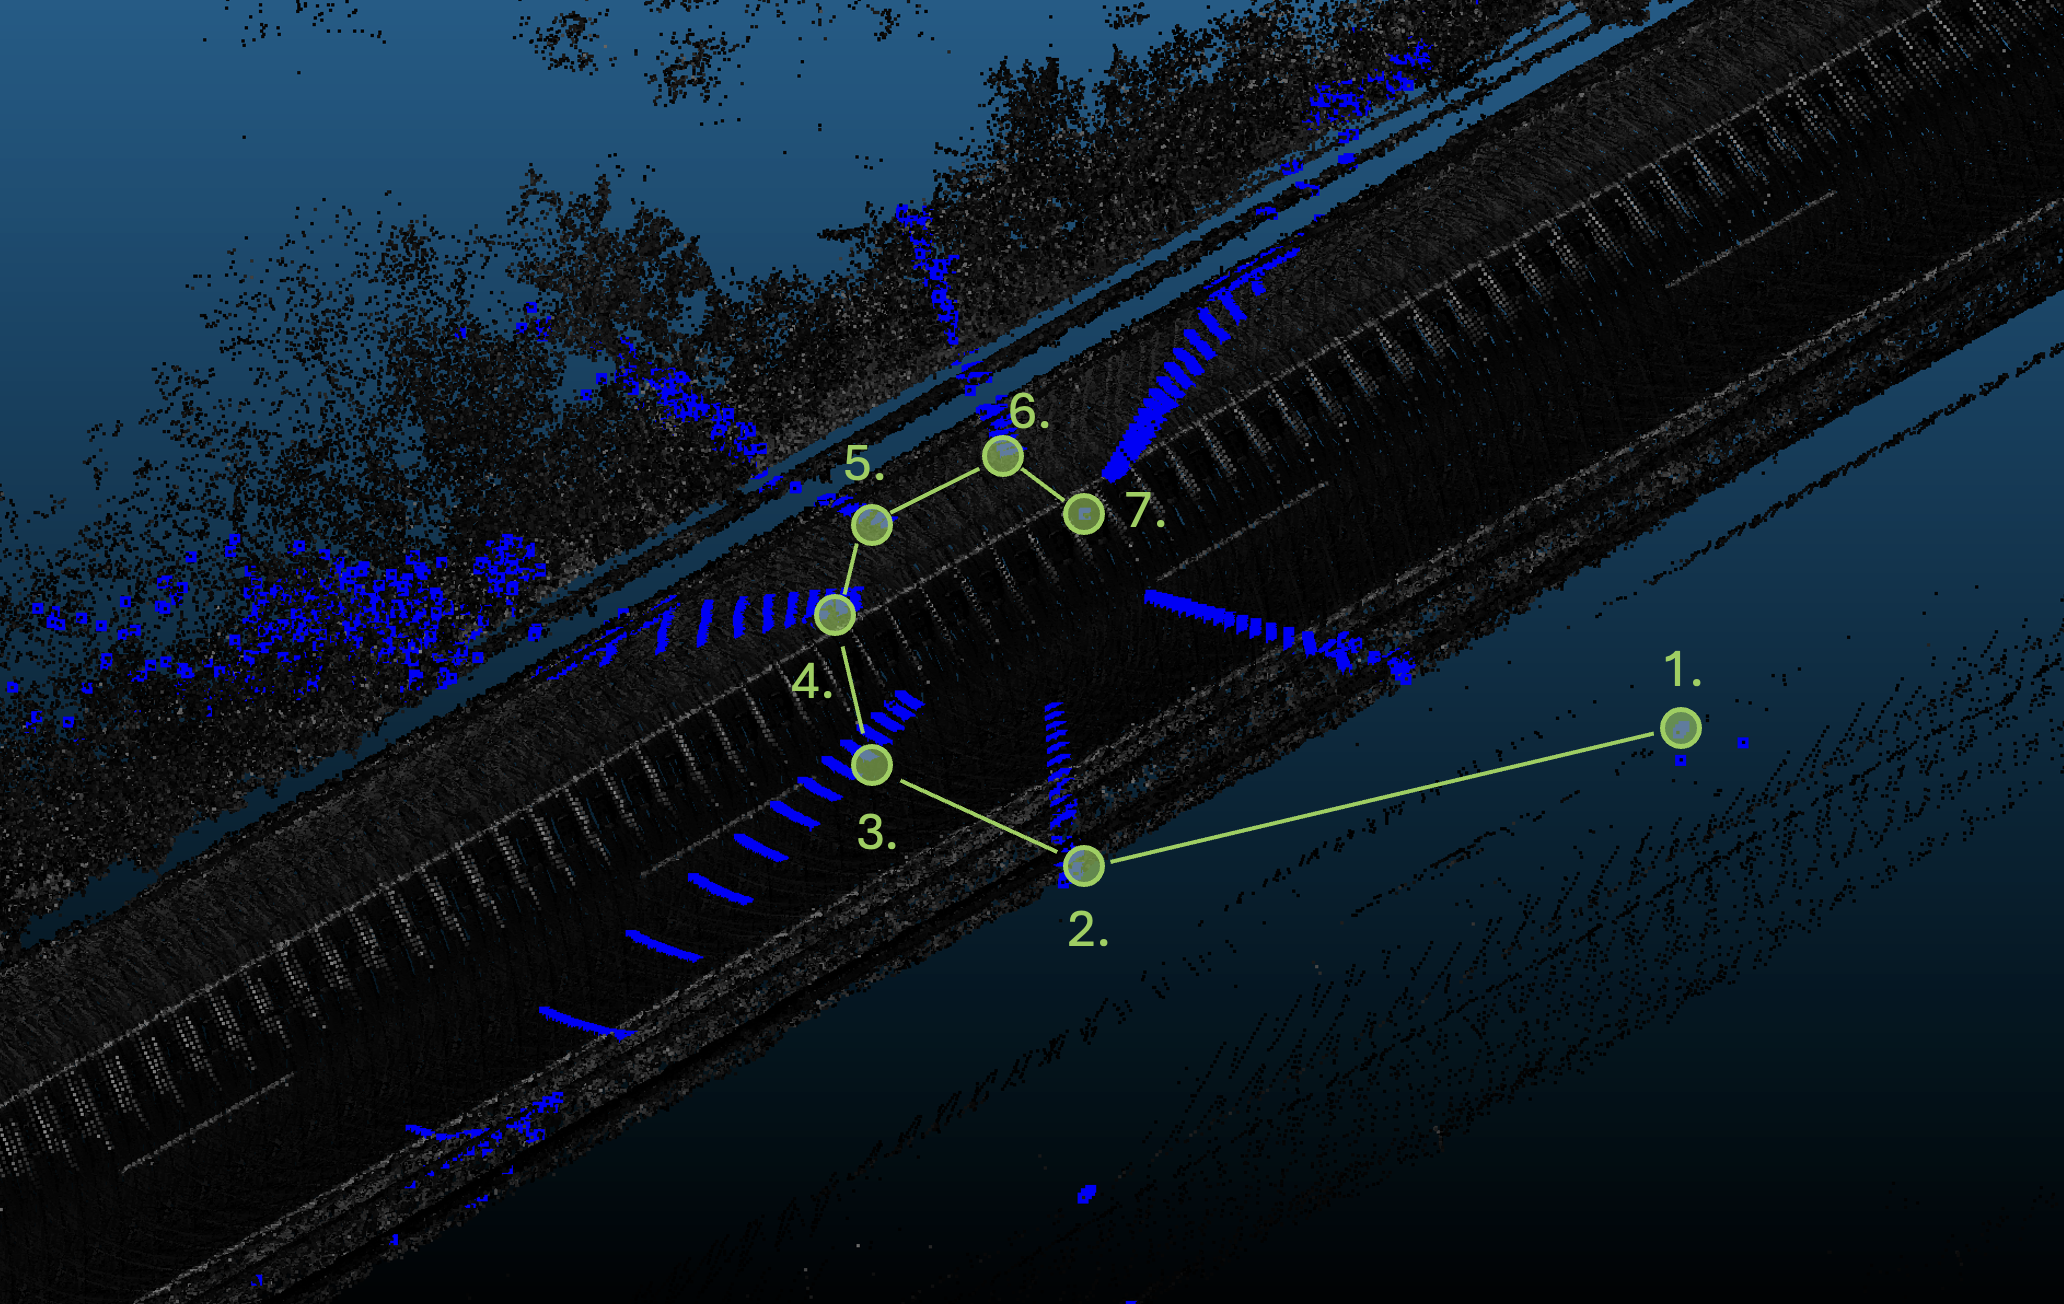
\includegraphics[width=\textwidth]{images/car_trace/closest_point_vis}
    \caption{Visualization of the iterative convergence process.}
    \label{fig:closest_point_vis}
  \end{subfigure}
  \hfill
  \begin{subfigure}[b]{0.48\textwidth}
    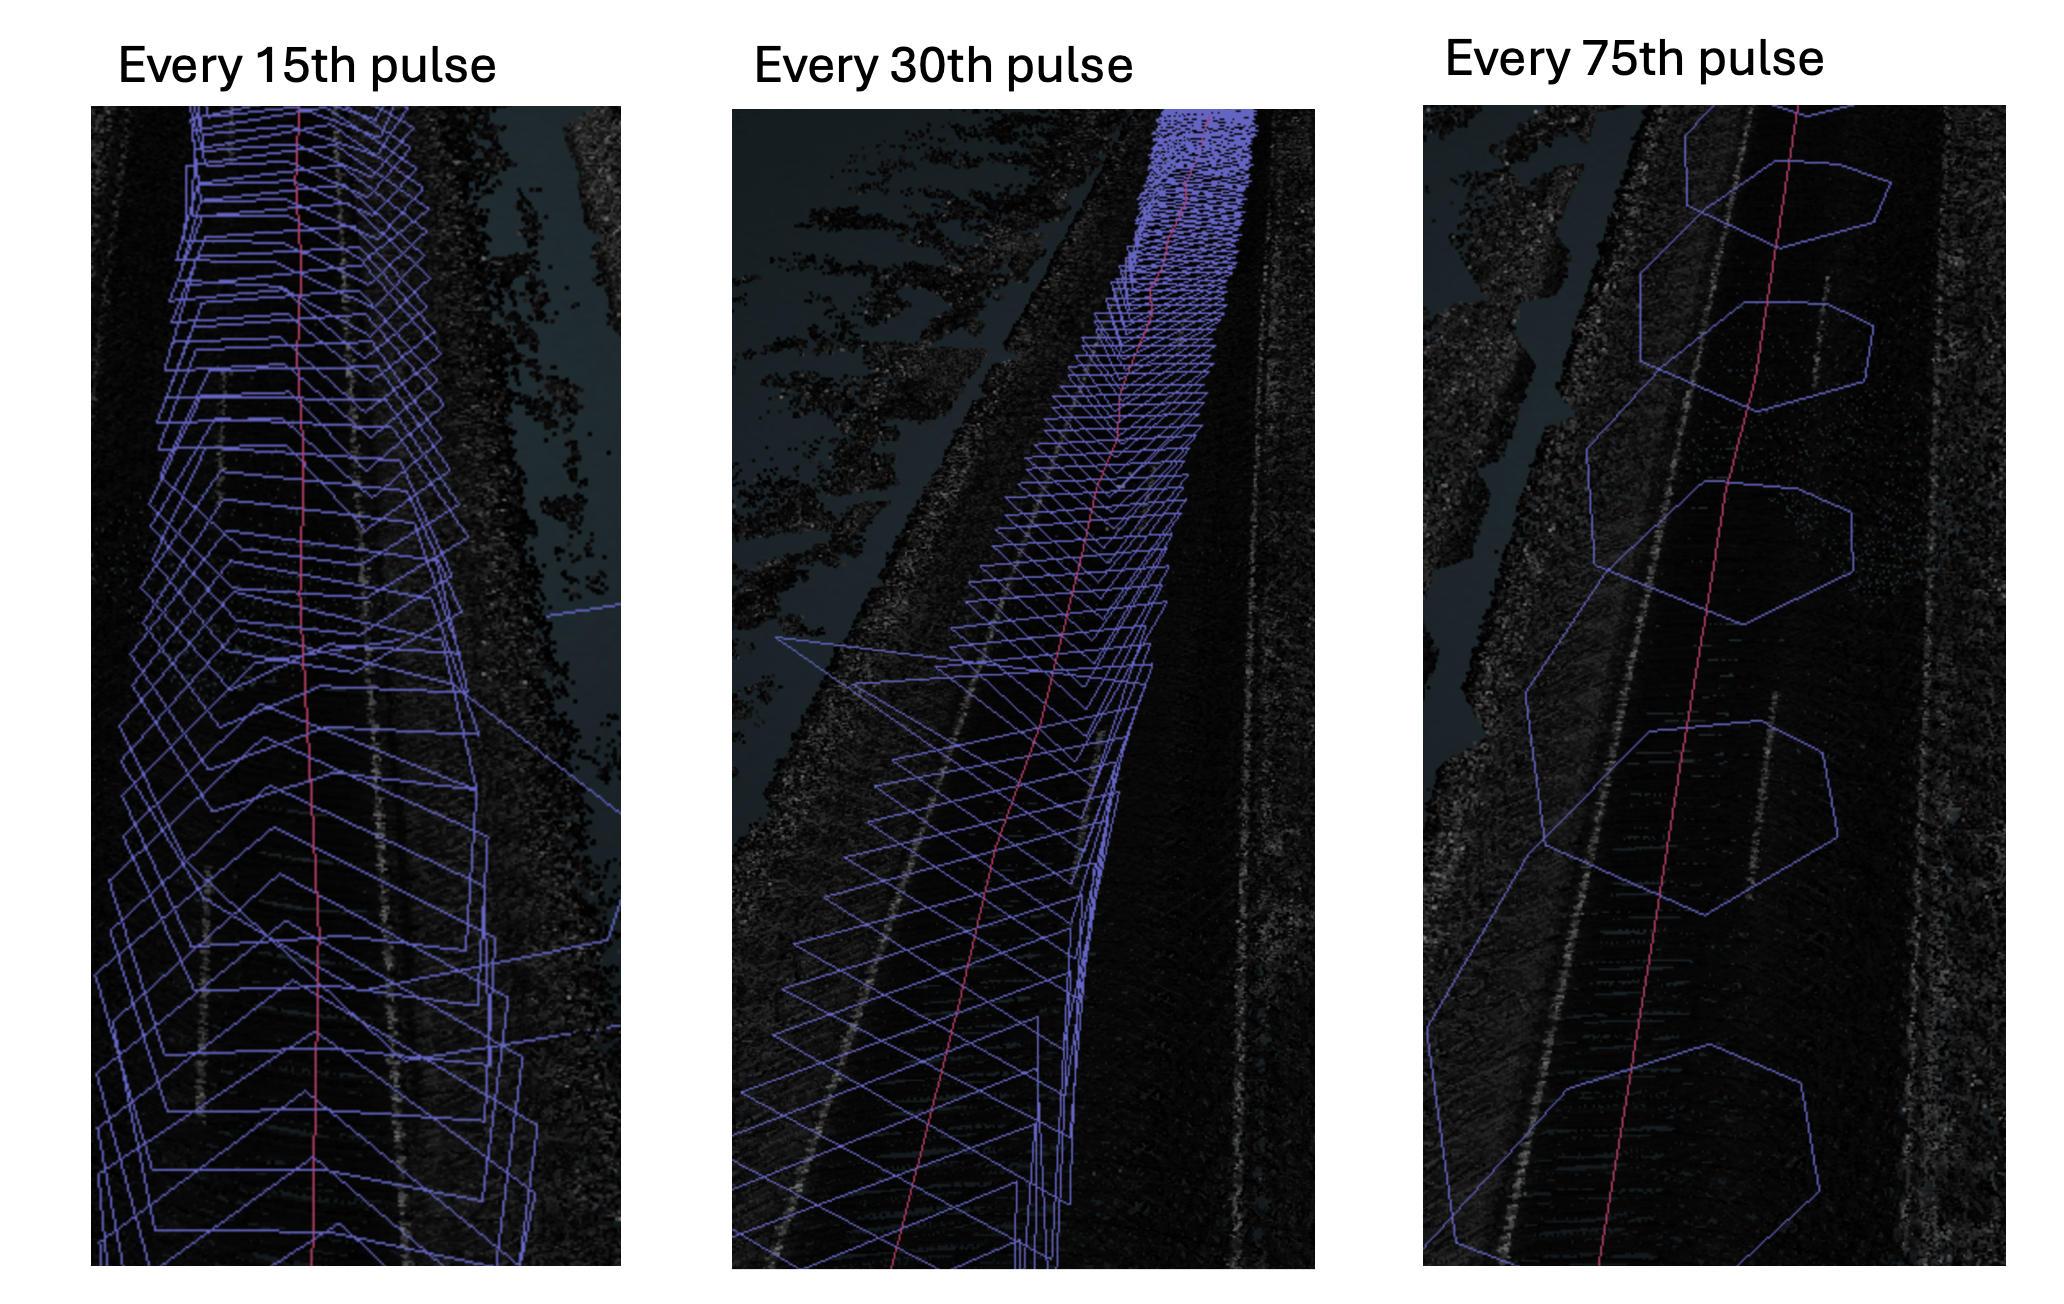
\includegraphics[width=\textwidth]{images/car_trace/closest_point_results}
    \caption{Output trajectory produced by the algorithm.}
    \label{fig:closest_point_results}
  \end{subfigure}
  \caption{The Closest Point Convergence algorithm: (a)~the iterative process by which successive estimates converge toward the sensor position; (b)~the resulting trajectory output.}
  \label{fig:closest_point}
\end{figure}

The output confirms that the convergence observation holds in practice. After applying a moving-window average followed by Gaussian smoothing, the resulting trajectory provides a usable estimate for subsequent pipeline stages.

\FloatBarrier
\subsection{Summary of Trajectory Reconstruction}
\label{sec:trace_summary}

Four trajectory reconstruction algorithms were presented, each providing adequate estimates under appropriate conditions. Table~\ref{tab:trace_algorithms} summarizes their characteristics. The pipeline uses the Pulse Line Intersection algorithm by default, as it consistently produced the most accurate estimates.

\begin{table}[htbp]
  \centering
  \caption{Summary of vehicle trajectory reconstruction algorithms.}
  \label{tab:trace_algorithms}
  \small
  \begin{tabular}{@{}lp{0.3\textwidth}p{0.35\textwidth}@{}}
    \hline
    Algorithm & Principle & Limitation \\
    \hline
    Window Median & Median of temporal window & Asymmetric reflection bias \\
    Window Median + GF & Ground-filtered median & Requires reasonable initial estimate \\
    Pulse Line Intersection & Regression line intersection & Requires sufficient angular separation \\
    Closest Point Convergence & Iterative nearest-point update & Requires post-processing (smoothing) \\
    \hline
  \end{tabular}
\end{table}

\FloatBarrier
%------------------------------------------------------------------
\section{Point Cloud Processing}
\label{sec:pointcloud_processing}

% TODO: This section will detail the following processing stages:
% - Binning along the vehicle trace
% - Distance-based clipping
% - RANSAC-based ground segmentation
% - Region-growing road surface detection
% - Intensity thresholding for road marking segmentation

\FloatBarrier
%------------------------------------------------------------------
\section{Line Fitting}
\label{sec:line_fitting}

% TODO: This section will detail the following stages:
% - Line extension RANSAC
% - Moving least squares refinement
% - Line labeling (solid vs. dashed)

\cleardoublepage

\chapter{Evaluation}
\label{ch:eval}

This chapter evaluates the two main algorithmic contributions of the pipeline: the vehicle trajectory reconstruction methods (Section~\ref{sec:eval_trace}) and the lane extraction pipeline (Section~\ref{sec:eval_lanes}).

\section{Ground Truth Collection}
\label{sec:eval_gt}

Ground truth data was manually collected for both evaluation tasks. The vehicle trajectory ground truth covers approximately $4700\,\mathrm{m}$ of the recorded highway segment. Collection was made possible by the fact that the LiDAR sensor captured a partial scan of the vehicle's trunk during every rotation. The centroids of these trunk point clusters were manually extracted and used as ground truth positions of the vehicle/sensor. Since this method need not be perfectly precise---only sufficiently accurate to serve as a reference for algorithm comparison---it provides an adequate basis for evaluation.

The lane geometry ground truth spans more than $10\,\mathrm{km}$ of annotated lane boundaries, each labeled semantically as either \emph{solid} or \emph{dashed}. The geometries were extracted based on intensity values and saved to a GeoPackage file.

%------------------------------------------------------------------
\section{Vehicle Trajectory Reconstruction Evaluation}
\label{sec:eval_trace}

\subsection{Evaluation Methodology}
\label{sec:eval_trace_method}

To quantitatively evaluate the geometric accuracy of the generated vehicle trajectories, the algorithm-produced traces were compared against the manually annotated ground-truth reference traces. The evaluation focuses on spatial similarity between the detected and reference paths and measures both average positional accuracy and worst-case deviations. The same evaluation procedure was applied to all four trajectory reconstruction methods.

\subsubsection{Spatial Alignment and Preprocessing}

Both the algorithm-generated trace and the ground-truth trace were loaded from GeoPackage files and transformed into the Hungarian projected coordinate reference system EPSG:23700. Using a projected CRS ensures that all geometric distance calculations are performed in metres.

Since the algorithms produce trajectories extending beyond the manually annotated road segment, the generated trace was spatially trimmed before comparison. The start and end points of the ground-truth trajectory were projected onto the generated polyline, and the corresponding substring was extracted. This step guarantees that both geometries represent the same road segment.

\subsubsection{Trajectory Sampling}

To enable dense geometric comparison, both polylines were sampled at regular intervals of $0.3\,\mathrm{m}$ along their lengths, producing approximately uniformly spaced points on each trajectory. Let
\begin{equation}
  G = \{g_1, g_2, \dots, g_n\}
  \label{eq:gt_samples}
\end{equation}
denote the sampled points of the ground-truth trajectory, and
\begin{equation}
  A = \{a_1, a_2, \dots, a_m\}
  \label{eq:algo_samples}
\end{equation}
the sampled points of the algorithm-generated trajectory.

\subsubsection{Bidirectional Point-to-Curve Distance Evaluation}

The evaluation computes distances in both directions:
\begin{enumerate}
  \item From every ground-truth sample point $g_i \in G$ to the generated trajectory $A$.
  \item From every generated sample point $a_j \in A$ to the ground-truth trajectory $G$.
\end{enumerate}

For a point $g_i \in G$, the distance to $A$ is defined as
\begin{equation}
  d(g_i, A) = \min_{a \in A} \|g_i - a\|,
  \label{eq:point_to_curve}
\end{equation}
and analogously for points sampled from $A$. Using bidirectional distances is important because a one-sided evaluation may fail to capture certain geometric discrepancies: a generated trajectory may fully cover the ground-truth line while also containing large overextensions elsewhere (see Figure~\ref{fig:trace_sampling}).

\begin{figure}[htbp]
  \centering
  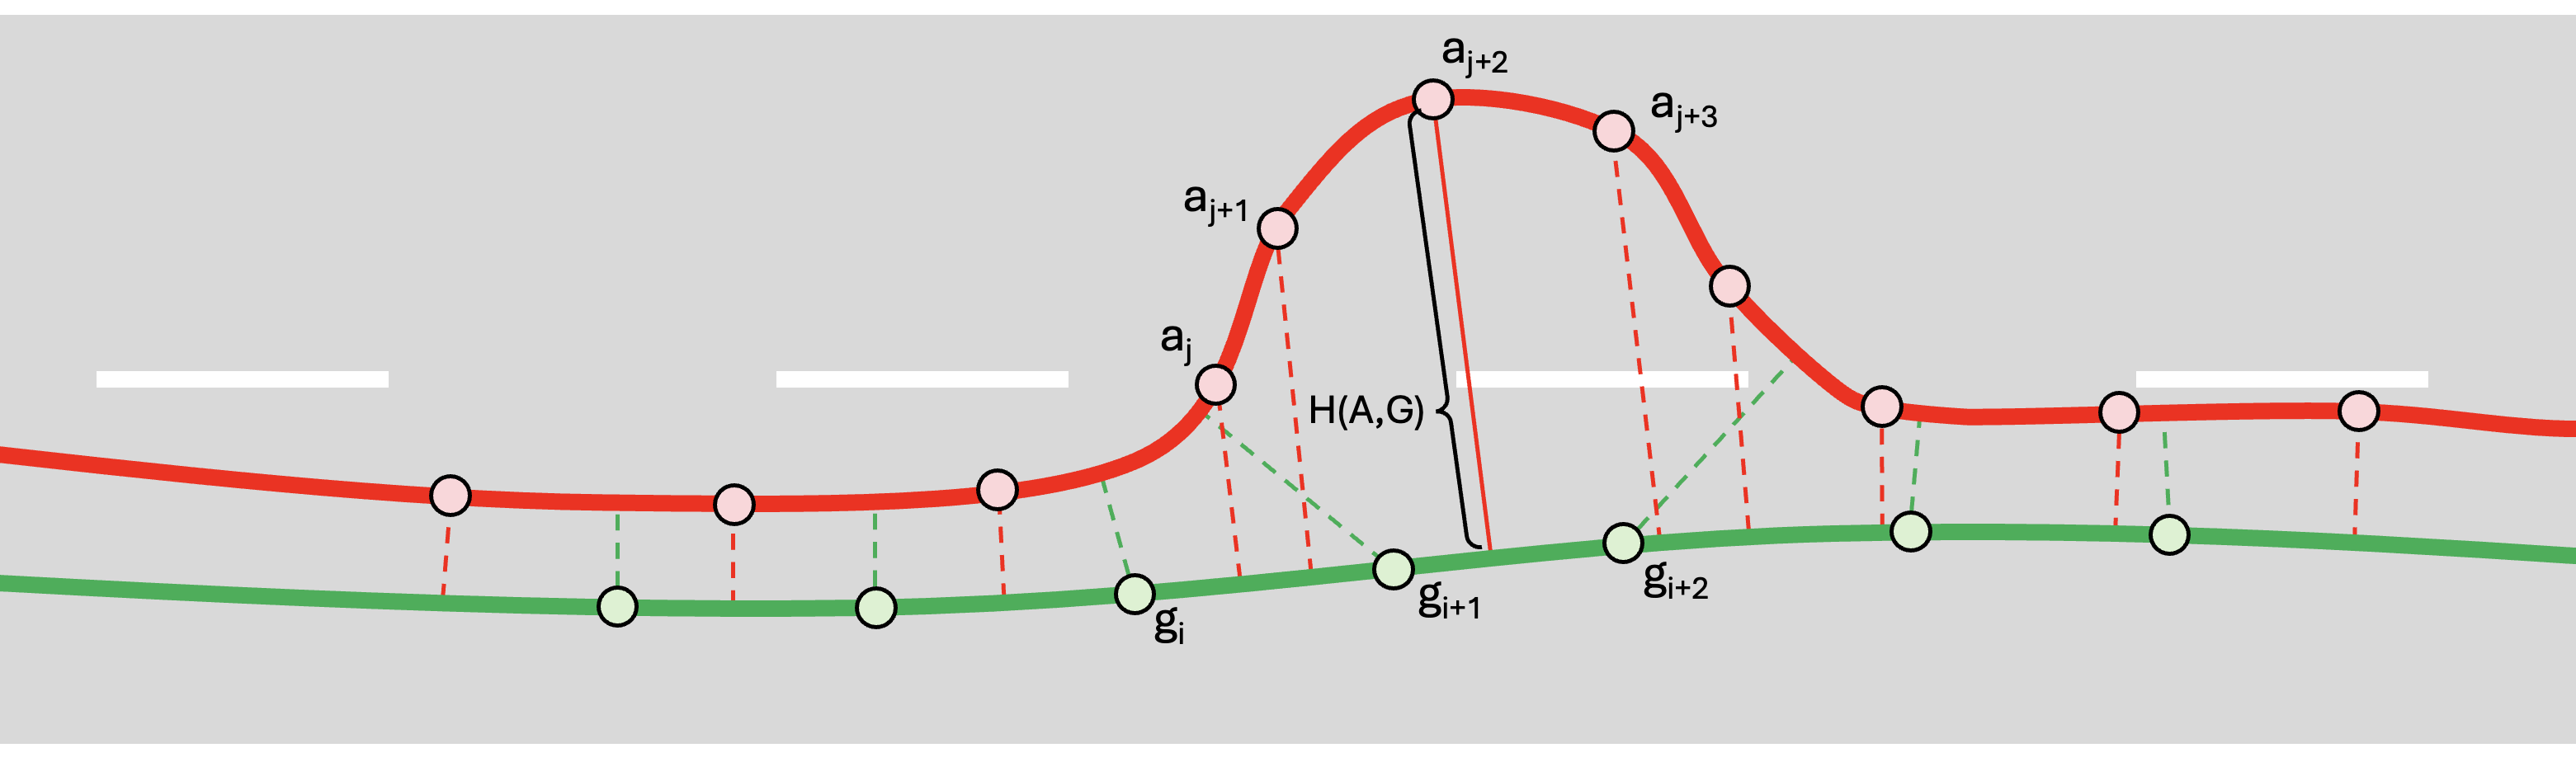
\includegraphics[width=0.8\textwidth]{images/evaluation/trace/trace_sampling}
  \caption{Illustration of the bidirectional sampling-based evaluation. Ground-truth trace (green) and algorithm trace (red) are sampled densely; shortest distances from green samples (light green) and from red samples (pink) are computed independently. The Hausdorff distance is the maximum of all shortest distances.}
  \label{fig:trace_sampling}
\end{figure}

For each direction, the following statistical measures were computed:

\begin{description}
  \item[Mean Error] Average geometric deviation between the trajectories:
    \begin{equation}
      \mu = \frac{1}{N}\sum_{i=1}^{N} d_i.
      \label{eq:mean_error}
    \end{equation}

  \item[Root Mean Square Error (RMSE)] Gives higher weight to larger local deviations:
    \begin{equation}
      \mathrm{RMSE} = \sqrt{\frac{1}{N}\sum_{i=1}^{N} d_i^2}.
      \label{eq:rmse}
    \end{equation}

  \item[95th Percentile (P95)] The distance below which $95\%$ of all sampled errors fall.

  \item[99th Percentile (P99)] Indicates the behavior of extreme outliers while remaining less sensitive than the absolute maximum.
\end{description}

\FloatBarrier
\subsection{Hausdorff Distance}
\label{sec:eval_hausdorff}

As a global similarity measure, the evaluation also computes the Hausdorff distance between the two trajectories. The directed Hausdorff distance from $A$ to $G$ is defined as
\begin{equation}
  h(A, G) = \max_{a \in A} \min_{g \in G} \|a - g\|,
  \label{eq:directed_hausdorff}
\end{equation}
and the symmetric Hausdorff distance is
\begin{equation}
  H(A, G) = \max\bigl(h(A, G),\; h(G, A)\bigr).
  \label{eq:hausdorff}
\end{equation}

Intuitively, the Hausdorff distance represents the largest local deviation between the two trajectories: it is the maximum distance that any point on one curve must travel to reach the nearest point on the other. Unlike mean-based metrics, it is highly sensitive to localized outliers and therefore provides a useful worst-case similarity measure. A small Hausdorff distance indicates that the generated trajectory remains close to the reference everywhere along its length.

\FloatBarrier
\subsection{Fréchet Distance}
\label{sec:eval_frechet}

Another commonly used curve similarity metric is the Fréchet distance, which---unlike the Hausdorff distance---takes the ordering of points along the curves into account. It is often illustrated by the analogy of a person walking a dog: both move along their respective curves without backtracking, and the Fréchet distance is the minimum leash length required. Formally, for two curves $f$ and $g$:
\begin{equation}
  F(f, g) = \inf_{\alpha,\beta}\; \max_{t \in [0,1]} \|f(\alpha(t)) - g(\beta(t))\|,
  \label{eq:frechet}
\end{equation}
where $\alpha$ and $\beta$ are continuous non-decreasing reparameterizations of the two curves.

Although the Fréchet distance is frequently used for trajectory comparison, it was not necessary in this evaluation because the trajectories contain no loops, self-intersections, or backward movements. Under such conditions, the Fréchet and Hausdorff distances tend to be very similar in practice, since both trajectories follow nearly monotonic paths with consistent ordering. In general,
\begin{equation}
  F(A, G) \geq H(A, G),
  \label{eq:frechet_hausdorff}
\end{equation}
with equality only in special cases. The Fréchet distance would therefore provide little additional information beyond the Hausdorff distance for these trajectories.

\FloatBarrier
\subsection{Evaluation Results}
\label{sec:eval_trace_results}

Tables~\ref{tab:trace_wm1}--\ref{tab:trace_cp} report the evaluation metrics for each trajectory reconstruction method. Figure~\ref{fig:trace_histograms} shows the corresponding distance distributions.

\begin{table}[htbp]
  \centering
  \caption{Window Median (Baseline) --- trajectory evaluation results.}
  \label{tab:trace_wm1}
  \small
  \begin{tabular}{@{}lrrrr@{}}
    \hline
    Direction   & Mean Error & RMSE    & P95     & P99     \\
    \hline
    GT $\to$ Algo & $0.653\,\mathrm{m}$ & $0.748\,\mathrm{m}$ & $1.252\,\mathrm{m}$ & $1.769\,\mathrm{m}$ \\
    Algo $\to$ GT & $0.653\,\mathrm{m}$ & $0.747\,\mathrm{m}$ & $1.250\,\mathrm{m}$ & $1.768\,\mathrm{m}$ \\
    \hline
    \multicolumn{2}{@{}l}{Hausdorff distance} & \multicolumn{3}{r@{}}{$1.960\,\mathrm{m}$} \\
    \hline
  \end{tabular}
\end{table}

\begin{table}[htbp]
  \centering
  \caption{Window Median with Ground Filtering (V2) --- trajectory evaluation results.}
  \label{tab:trace_wm2}
  \small
  \begin{tabular}{@{}lrrrr@{}}
    \hline
    Direction   & Mean Error & RMSE    & P95     & P99     \\
    \hline
    GT $\to$ Algo & $0.177\,\mathrm{m}$ & $0.305\,\mathrm{m}$ & $0.508\,\mathrm{m}$ & $1.527\,\mathrm{m}$ \\
    Algo $\to$ GT & $0.176\,\mathrm{m}$ & $0.303\,\mathrm{m}$ & $0.506\,\mathrm{m}$ & $1.522\,\mathrm{m}$ \\
    \hline
    \multicolumn{2}{@{}l}{Hausdorff distance} & \multicolumn{3}{r@{}}{$1.782\,\mathrm{m}$} \\
    \hline
  \end{tabular}
\end{table}

\begin{table}[htbp]
  \centering
  \caption{Pulse Line Intersection --- trajectory evaluation results.}
  \label{tab:trace_pl}
  \small
  \begin{tabular}{@{}lrrrr@{}}
    \hline
    Direction   & Mean Error & RMSE    & P95     & P99     \\
    \hline
    GT $\to$ Algo & $0.147\,\mathrm{m}$ & $0.182\,\mathrm{m}$ & $0.348\,\mathrm{m}$ & $0.439\,\mathrm{m}$ \\
    Algo $\to$ GT & $0.147\,\mathrm{m}$ & $0.183\,\mathrm{m}$ & $0.349\,\mathrm{m}$ & $0.439\,\mathrm{m}$ \\
    \hline
    \multicolumn{2}{@{}l}{Hausdorff distance} & \multicolumn{3}{r@{}}{$0.725\,\mathrm{m}$} \\
    \hline
  \end{tabular}
\end{table}

\begin{table}[htbp]
  \centering
  \caption{Closest Point Convergence (after smoothing) --- trajectory evaluation results.}
  \label{tab:trace_cp}
  \small
  \begin{tabular}{@{}lrrrr@{}}
    \hline
    Direction   & Mean Error & RMSE    & P95     & P99     \\
    \hline
    GT $\to$ Algo & $0.653\,\mathrm{m}$ & $0.748\,\mathrm{m}$ & $1.252\,\mathrm{m}$ & $1.769\,\mathrm{m}$ \\
    Algo $\to$ GT & $0.653\,\mathrm{m}$ & $0.747\,\mathrm{m}$ & $1.250\,\mathrm{m}$ & $1.768\,\mathrm{m}$ \\
    \hline
    \multicolumn{2}{@{}l}{Hausdorff distance} & \multicolumn{3}{r@{}}{$1.960\,\mathrm{m}$} \\
    \hline
  \end{tabular}
\end{table}

\begin{figure}[htbp]
  \centering
  \begin{subfigure}[b]{0.8\textwidth}
    \centering
    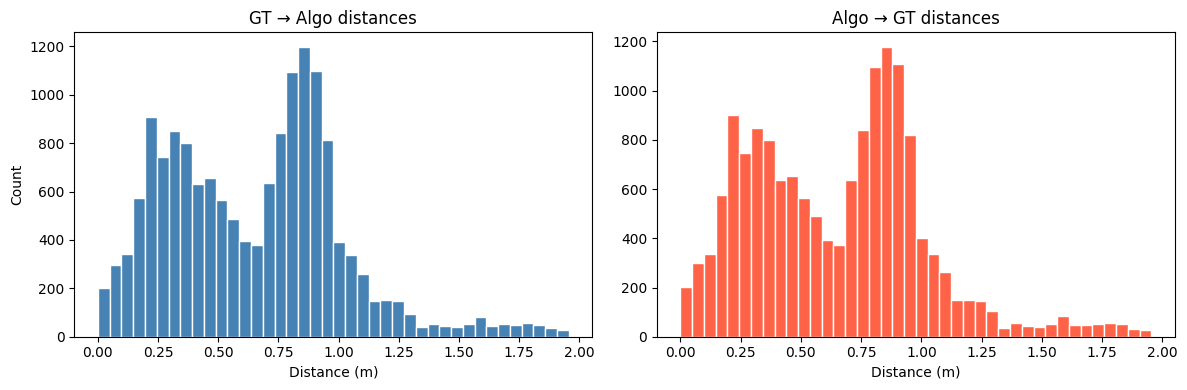
\includegraphics[width=\textwidth]{images/evaluation/trace/hist_wm1}
    \caption{Window Median (Baseline).}
    \label{fig:hist_wm1}
  \end{subfigure}
  \\[0.5em]
  \begin{subfigure}[b]{0.8\textwidth}
    \centering
    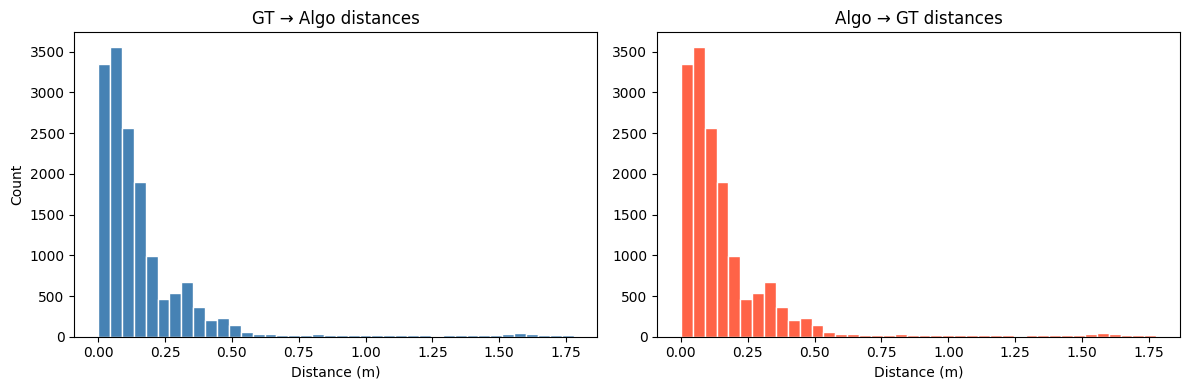
\includegraphics[width=\textwidth]{images/evaluation/trace/hist_wm2}
    \caption{Window Median with Ground Filtering (V2).}
    \label{fig:hist_wm2}
  \end{subfigure}
  \\[0.5em]
  \begin{subfigure}[b]{0.8\textwidth}
    \centering
    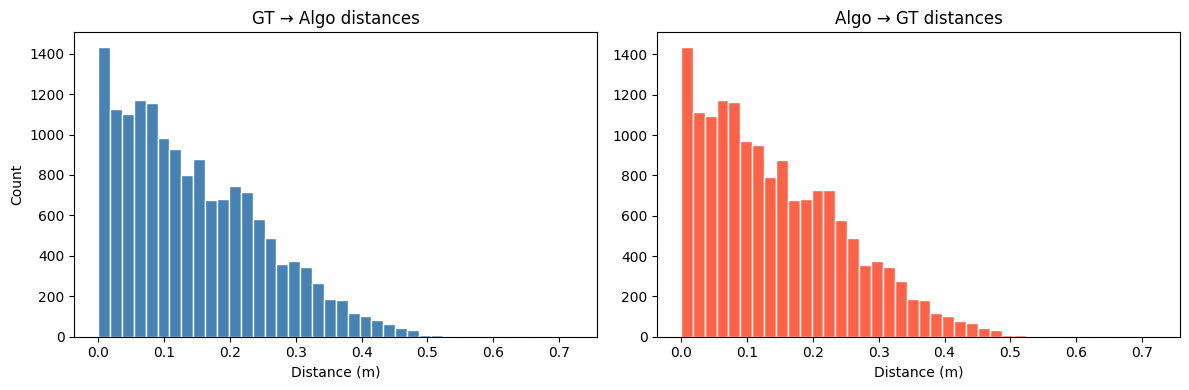
\includegraphics[width=\textwidth]{images/evaluation/trace/hist_pl}
    \caption{Pulse Line Intersection.}
    \label{fig:hist_pl}
  \end{subfigure}
  \\[0.5em]
  \begin{subfigure}[b]{0.8\textwidth}
    \centering
    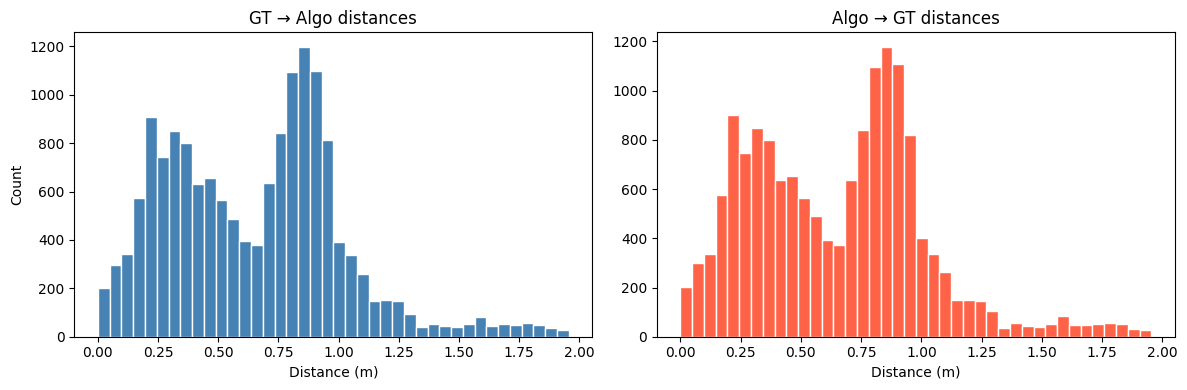
\includegraphics[width=\textwidth]{images/evaluation/trace/hist_cp}
    \caption{Closest Point Convergence.}
    \label{fig:hist_cp}
  \end{subfigure}
  \caption{Distance distribution histograms for all four trajectory reconstruction algorithms. Left: distances from ground-truth sample points to the algorithm trace ($G \to A$); right: distances from algorithm sample points to the ground-truth trace ($A \to G$).}
  \label{fig:trace_histograms}
\end{figure}

\FloatBarrier
\subsection{Summary}
\label{sec:eval_trace_summary}

Among the evaluated methods, the Pulse Line Intersection algorithm achieved the best overall geometric accuracy, with the lowest mean error ($0.147\,\mathrm{m}$), lowest RMSE ($0.182\,\mathrm{m}$), lowest percentile errors, and the smallest Hausdorff distance ($0.725\,\mathrm{m}$). The Window Median V2 algorithm showed a substantial improvement over the baseline Window Median, particularly in average error metrics. The baseline Window Median and Closest Point approaches produced significantly larger deviations, with identical metrics in this evaluation, and higher worst-case errors. These results confirm the selection of Pulse Line Intersection as the default trajectory reconstruction method in the pipeline.

%------------------------------------------------------------------
\section{Lane Extraction Evaluation}
\label{sec:eval_lanes}

\subsection{Evaluated Configurations}
\label{sec:eval_lanes_configs}

To assess the sensitivity of the lane extraction pipeline to key parameters, four configurations were evaluated:

\begin{enumerate}
  \item \textbf{Baseline}: default parameter configuration.
  \item \textbf{Bin\_40}: bin length increased from $25\,\mathrm{units}$ to $40\,\mathrm{units}$.
  \item \textbf{Intensity\_10}: intensity threshold percentile increased from $5\%$ to $10\%$.
  \item \textbf{Intensity\_Kapur}: percentile-based intensity thresholding replaced with max-entropy entropy thresholding.
\end{enumerate}

\paragraph{Note on bin-length units.}\mbox{} \\
The \texttt{bin\_length} parameter is expressed in the native coordinate units of the input point cloud, without any internal reprojection.
In this experiment the input LiDAR data was stored in EPSG:3857 (Web Mercator), whose units are pseudo-metres: at the latitude of the study area (approximately $47^{\circ}$N) the scale factor is $\sec(47^{\circ}) \approx 1.47$, so distances are stretched by roughly $47\%$ relative to true ground distances.
Consequently, the configured values of $25$ and $40$ correspond to approximately $17\,\mathrm{m}$ and $27\,\mathrm{m}$ of actual ground distance, respectively.
Had the input data been provided in a local projected CRS, the same parameter values would directly represent metres on the ground.
All evaluation metrics reported in this chapter are computed after reprojection to EPSG:23700 and therefore reflect true metric distances.

All other pipeline stages and parameters---including input point cloud, temporal window configuration, ground segmentation, road-surface filtering, downsampling, RANSAC line fitting, line smoothing, lane labeling, and output settings---remained identical across all four experiments. This controlled setup ensures that observed performance differences can be attributed directly to the modified parameter.

\subsection{Evaluation Procedure}
\label{sec:eval_lanes_method}

\subsubsection{Cross-Section-Based Matching}

The evaluation compares predicted and ground-truth lane markings using a cross-sectional analysis approach. A set of evenly distributed cross-sections is generated perpendicular to the driving direction along the road segment. For each cross-section, intersections with both the predicted and ground-truth lane lines are computed.

Predicted and ground-truth intersections are then spatially matched based on proximity: a predicted intersection is considered a true positive if it falls within $20\,\mathrm{cm}$ of a ground-truth intersection. This approach evaluates performance at the level of individual lane-marker crossings rather than entire polylines, which directly measures lane count consistency, lateral positional accuracy, and lane-type classification quality. A total of 467 cross-sections were evaluated in each experiment.

\begin{figure}[htbp]
  \centering
  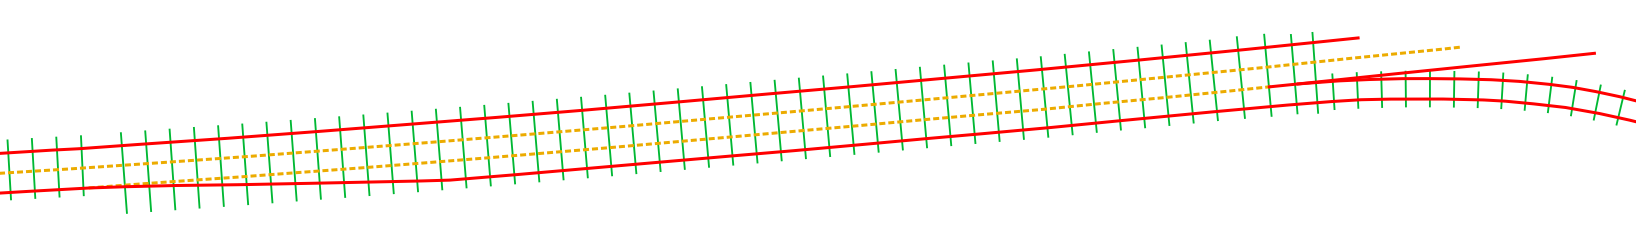
\includegraphics[width=0.7\textwidth]{images/evaluation/lanes/ground_truth_cross_sections}
  \caption{Ground-truth lane geometries: solid lane markings (continuous red), dashed lane markings (dashed orange). The evaluated cross-sections are displayed in green.}
  \label{fig:lbem_cross_section}
\end{figure}

\subsubsection{Detection Metrics}

The following detection metrics were computed from the matched intersections:
\begin{description}
  \item[True Positives (TP)] Predicted intersections correctly matched to a ground-truth intersection.
  \item[False Positives (FP)] Predicted intersections not matched to any ground-truth intersection.
  \item[False Negatives (FN)] Ground-truth intersections not matched by any prediction.
\end{description}

From these counts, standard information-retrieval metrics were derived:
\begin{equation}
  \mathrm{Precision} = \frac{TP}{TP + FP}, \qquad
  \mathrm{Recall} = \frac{TP}{TP + FN}, \qquad
  F_1 = 2 \cdot \frac{\mathrm{Precision} \cdot \mathrm{Recall}}{\mathrm{Precision} + \mathrm{Recall}}.
  \label{eq:prf1}
\end{equation}

\subsubsection{Geometric Accuracy Metrics}

For all matched intersection pairs, the Euclidean distance $d_i$ between the predicted and ground-truth positions was computed. The following statistics were evaluated:
\begin{equation}
  \mu = \frac{1}{N}\sum_{i=1}^{N} d_i, \qquad
  \mathrm{RMSE} = \sqrt{\frac{1}{N}\sum_{i=1}^{N} d_i^2}.
  \label{eq:lane_geo}
\end{equation}
Additionally, the median error, 95th percentile error (P95), and maximum error were reported.

\subsubsection{Lane Classification and Topological Metrics}

Each matched pair was compared by semantic class (solid or dashed). Classification accuracy measures, among the spatially matched intersection pairs, the fraction whose predicted lane type (solid or dashed) agrees with the ground-truth label:
\begin{equation}
  \mathrm{Acc}_{\mathrm{class}} = \frac{|\{i : \hat{y}_i = y_i\}|}{TP},
  \label{eq:class_acc}
\end{equation}
where $\hat{y}_i$ is the predicted semantic class and $y_i$ is the ground-truth class of the $i$-th matched pair. Purely spatial proximity is not sufficient for a correct prediction: the lane type must also match. For topological consistency, the lane count mean absolute error (MAE) was computed:
\begin{equation}
  \mathrm{MAE}_{\mathrm{count}} = \frac{1}{N}\sum_{i=1}^{N} |p_i - g_i|,
  \label{eq:lane_count_mae}
\end{equation}
where $p_i$ and $g_i$ denote the predicted and ground-truth lane counts at cross-section~$i$. The percentage of cross-sections where $p_i = g_i$ exactly (perfect cross-sections) was also reported.

\FloatBarrier
\subsection{Evaluation Results}
\label{sec:eval_lanes_results}

Table~\ref{tab:lane_eval} summarizes the evaluation results for all four configurations.

\begin{table}[htbp]
  \centering
  \caption{Lane extraction evaluation results across the four parameter configurations.}
  \label{tab:lane_eval}
  \small
  \begin{tabular}{@{}lrrrr@{}}
    \hline
    Metric & Baseline & Bin\_40 & Intensity\_10 & Intensity\_Kapur \\
    \hline
    TP                            & 1374   & 1348   & 1360   & 1374   \\
    FP                            & 1      & 13     & 14     & 4      \\
    FN                            & 20     & 46     & 34     & 20     \\
    Precision                     & 0.9993 & 0.9904 & 0.9898 & 0.9971 \\
    Recall                        & 0.9857 & 0.9670 & 0.9756 & 0.9857 \\
    $F_1$                         & 0.9924 & 0.9786 & 0.9827 & 0.9913 \\
    \hline
    Mean error (m)                & 0.0213 & 0.0221 & 0.0228 & 0.0220 \\
    RMSE (m)                      & 0.0280 & 0.0293 & 0.0307 & 0.0292 \\
    Median error (m)              & 0.0166 & 0.0175 & 0.0172 & 0.0173 \\
    P95 error (m)                 & 0.0564 & 0.0593 & 0.0589 & 0.0585 \\
    Max error (m)                 & 0.1750 & 0.1791 & 0.1832 & 0.1754 \\
    \hline
    Classification accuracy       & 0.9993 & 0.9993 & 0.9971 & 0.9993 \\
    Lane count MAE                & 0.0407 & 0.0707 & 0.0428 & 0.0471 \\
    Perfect cross-sections (\%)   & 96.36  & 93.15  & 96.15  & 95.72  \\
    Cross-sections                & 467    & 467    & 467    & 467    \\
    \hline
  \end{tabular}
\end{table}

\FloatBarrier
\subsection{Discussion}
\label{sec:eval_lanes_discussion}

The baseline configuration achieved the best overall performance across nearly all evaluation metrics: highest $F_1$ score ($0.9924$), lowest geometric errors, lowest lane-count MAE ($0.0407$), and the highest percentage of perfectly reconstructed cross-sections ($96.36\%$). These results indicate that the original parameter configuration provides the best balance between detection sensitivity, geometric precision, and topological consistency.

\begin{figure}[htbp]
  \centering
  \begin{subfigure}[b]{0.85\textwidth}
    \centering
    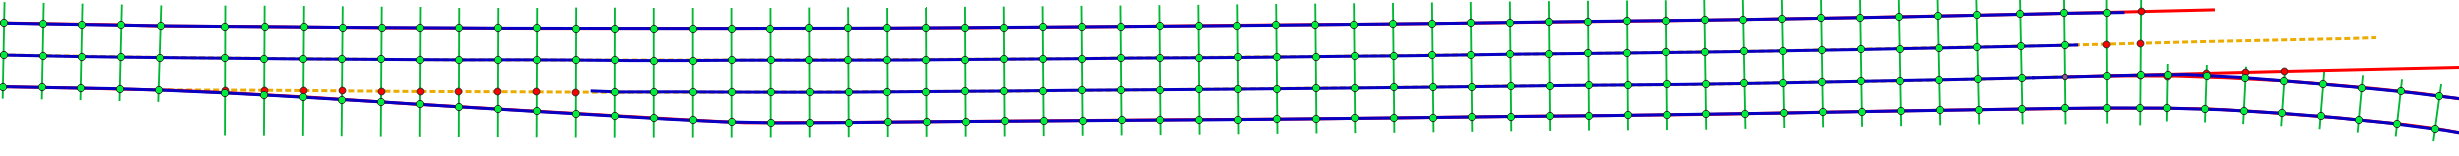
\includegraphics[width=\textwidth]{images/evaluation/lanes/eval_points}
    \caption{A road section where lane lines merge and split: the line-fitting stage cannot correctly handle such topological changes, resulting in false negatives.}
    \label{fig:eval_points_merge}
  \end{subfigure}
  \\[0.5em]
  \begin{subfigure}[b]{0.85\textwidth}
    \centering
    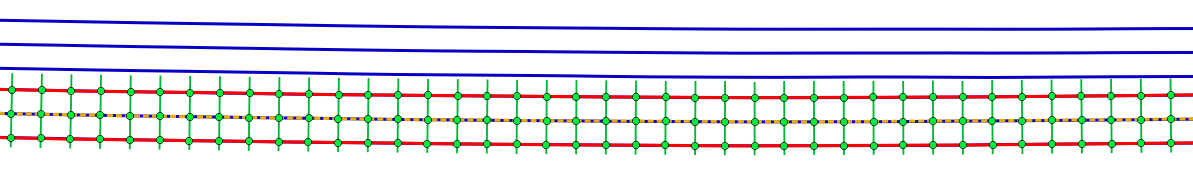
\includegraphics[width=\textwidth]{images/evaluation/lanes/eval_points_2}
    \caption{A typical highway section with no merging or splitting: all four configurations performed well under these ordinary conditions.}
    \label{fig:eval_points_normal}
  \end{subfigure}
  \caption{Qualitative evaluation results. Ground-truth solid markings (solid red), ground-truth dashed markings (dashed orange), extracted lane geometries (blue); true positives with correct semantic match (green dots), false negatives (red dots).}
  \label{fig:eval_points}
\end{figure}

The Kapur thresholding configuration (\textit{Intensity\_Kapur}) produced performance very close to the baseline. Although it introduced slightly more false positives (4 vs.\ 1), recall remained identical, and the geometric accuracy degradation was minimal. This suggests that entropy-based thresholding is a viable alternative to percentile-based intensity filtering and may be preferable in scenarios where the intensity distribution is less predictable.

Increasing the intensity percentile threshold to $10\%$ (\textit{Intensity\_10}) reduced detection quality: more false positives and false negatives were produced, leading to lower precision ($0.9898$), recall ($0.9756$), and $F_1$ score ($0.9827$). Geometric error metrics also increased slightly, indicating that the higher threshold likely suppresses valid lane marking points while retaining noise, making accurate line fitting more difficult.

The weakest performance was observed in the increased bin-length configuration (\textit{Bin\_40}). Enlarging the temporal bin length from $25$ to $40$ Web Mercator pseudo-metres (approximately $17\,\mathrm{m}$ to $27\,\mathrm{m}$ on the ground) substantially reduced recall ($0.9670$) and introduced the most false positives and lane-count inconsistencies. The decrease in perfect cross-sections ($93.15\%$) and the increased lane-count MAE ($0.0707$) indicate degraded topological reconstruction quality. This suggests that larger binning regions reduce the pipeline's ability to adapt to local road geometry variations and lane-structure changes.

Overall, the experiments demonstrate that the pipeline is highly sensitive to the binning configuration and moderately sensitive to intensity-threshold selection. Across all tested configurations, the baseline achieves sub-centimetre mean positional accuracy ($2.1\,\mathrm{cm}$) and near-perfect lane detection ($F_1 > 0.99$), confirming the effectiveness of the proposed lane extraction approach.

\FloatBarrier
\section{Performance and Resource Usage}
\label{sec:eval_performance}

All experiments were executed on an Apple MacBook Pro (Mac15,7) with an Apple M3 Pro SoC containing 12 CPU cores (6 performance and 6 efficiency cores) and $36,\mathrm{GB}$ of unified memory.

\subsection{Stage-wise Runtime}
Table~\ref{tab:stage_times} reports the average runtime (over 10 runs) for each pipeline stage when processing a typical highway segment.

\begin{table}[htbp]
  \centering
  \caption{Average runtime per pipeline stage (10 runs).}
  \label{tab:stage_times}
  \small
  \begin{tabular}{@{}lr@{}}
    \hline
    \textbf{Stage} & \textbf{Time (s)} \\
    \hline
    Setup Stage & 2.45 \\
    Car Trace Stage & 4.56 \\
    Binning Stage (1st) & 15.29 \\
    TraceDistanceFilterStage & 0.90 \\
    GroundSegmentStage & 14.18 \\
    IntensityThresholdStage & 11.22 \\
    RoadSurfaceFilter & 4.85 \\
    DownsampleStage & 3.32 \\
    Binning Stage (2nd) & 0.07 \\
    FitLinesStage & 10.47 \\
    LineSmoothingStage & 16.41 \\
    LineLabelingStage & 31.19 \\
    \hline
  \end{tabular}
\end{table}

The total runtime for a full pipeline execution is approximately 115 seconds (just under 2 minutes) for a ~5 km highway segment, and more than 100 million points.

\subsection{Point Cloud Size Reduction}
The pipeline achieves substantial data reduction through progressive filtering and downsampling. Table~\ref{tab:point_reduction} shows the number of points remaining after each major stage for the sample tile 871e1d886ffffff.

\begin{table}[htbp]
  \centering
  \caption{Point count after each major processing stage (tile 871e1d886ffffff).}
  \label{tab:point_reduction}
  \small
  \begin{tabular}{@{}lr@{}}
    \hline
    \textbf{Stage} & \textbf{Points Remaining} \\
    \hline
    Raw input & 104,028,999 \\
    Distance clip & 81,139,327 \\
    Ground segmentation & 60,822,026 \\
    Intensity thresholding & 3,317,369 \\
    Road surface extraction & 894,671 \\
    Downsampling & 342,185 \\
    \hline
  \end{tabular}
\end{table}

This reduction enables efficient downstream processing and storage, while preserving all relevant lane geometry information.

\cleardoublepage

\chapter{Limitations and Future Work}
\label{ch:future}

\section{Limitations}
\label{sec:limitations}

Although the proposed pipeline produced accurate lane boundary geometries on the evaluated highway datasets, several limitations remain.

One important limitation is the reliance on manually defined parameters throughout multiple stages of the pipeline.
While some parameters primarily influence computational efficiency, others significantly affect the geometric quality of the extracted lanes.

For example, the distance-based clipping threshold mainly impacts runtime performance.
As long as the clipping radius is sufficiently large to fully contain the roadway, the final geometric output remains largely unchanged.
However, selecting unnecessarily large values substantially increases computational cost due to the increased number of processed points.

In contrast, the intensity thresholding stage is highly sensitive to parameter selection.
As demonstrated in Section~\ref{sec:eval_lanes}, the chosen threshold strongly influences the balance between false positives and false negatives.
Low thresholds preserve lane markings but admit large amounts of noise from reflective vegetation and surrounding structures, while high thresholds suppress noise at the cost of removing genuine lane marking points.
Although localized window-based thresholding improves robustness, the threshold selection still depends heavily on the characteristics of the environment, pavement material, and lane marking quality.

Additional manually tuned parameters appear in the line fitting and labeling stages.
These include the maximum distance between points and fitted lines, clustering thresholds, minimum segment lengths, and the rules used to distinguish solid and dashed lane boundaries.
The optimal values for these parameters may vary across environments and sensor configurations, limiting the generalizability of the current implementation.

Consequently, the proposed pipeline currently requires environment-specific parameter tuning and has primarily been validated on highway datasets with relatively regular geometries and clearly visible lane markings.
Its robustness in highly heterogeneous urban environments remains an open question.

\section{Future Work}
\label{sec:future_work}

Several promising directions exist for future work.

One extension would involve extracting additional semantic road marking information beyond lane boundaries.
The current pipeline focuses primarily on continuous lane geometries, but the same processing framework could potentially be extended to detect and reconstruct arrows, stop lines, text markings, and other road surface symbols.

Another important direction is the use of the pipeline for generating high-quality training datasets for machine learning and deep learning approaches.
Since the proposed method operates directly on raw LiDAR point clouds and produces geometrically accurate vectorized outputs, it could provide large-scale pseudo-ground-truth annotations for supervised learning systems.
Such datasets could support the development of more robust multi-scene perception models capable of handling faded lane markings, intersections, occlusions, and context-dependent road geometries.

Future research should also investigate hybrid approaches combining the deterministic geometric pipeline with learning-based semantic understanding.
In complex urban environments, lane geometries are often only partially visible, requiring inference from contextual information such as surrounding traffic infrastructure, road topology, and neighbouring lane configurations.

Finally, the proposed pipeline should be integrated into large-scale production workflows and evaluated on significantly larger and more diverse datasets.
Running the system on substantially more recording sessions would allow verification of its robustness across varying environmental conditions, road types, pavement materials, and sensor characteristics.
In addition, the generated lane geometries should be quantitatively compared against manually annotated ground truth using industrial in-house HD map quality metrics such as Absolute Positional Accuracy (APA) and Relative Positional Accuracy (RPA).
Such large-scale validation would provide a more complete assessment of the practical applicability of the proposed methodology in production-grade HD mapping systems.

\cleardoublepage

% Acknowledgements (optional) - in case your thesis received funding or would like to express special thanks to someone
\chapter*{\acklabel}
\addcontentsline{toc}{chapter}{\acklabel}

I would like to express my gratitude to TomTom N.V.~for the opportunity to work on this interesting topic within their Maps Advanced Analytics division.
Their provision of hardware infrastructure, LiDAR datasets, and a stimulating research environment were instrumental in making this thesis possible.

\ifUPM\else
I am also grateful to my internal supervisor, Hajder Levente, for his patient guidance, insightful feedback, and support throughout the research and writing process.

My friend Dávid deserves special thanks for his encouragement during the most challenging periods of this work, providing both moral support and perspective when needed.

\fi
Most importantly, I wish to extend my heartfelt appreciation to both my Mother and Father.
Their constant support, encouragement, and belief in me throughout all my life and studies have been the foundation upon which this achievement stands.
This thesis is, in many ways, a reflection of their dedication and love.


% Appendices (optional) - useful for detailed information in long tables, many and/or large figures, etc.
\appendix
% \input{chapters/appendix.tex}
% \cleardoublepage

% Bibliography (mandatory)
\phantomsection
\addcontentsline{toc}{chapter}{\biblabel}
\printbibliography[title=\biblabel]
\cleardoublepage

% List of figures (optional) - useful over 3-5 figures
% \phantomsection
% \addcontentsline{toc}{chapter}{\lstfigurelabel}
% \listoffigures
% \cleardoublepage

% List of tables (optional) - useful over 3-5 tables
% \phantomsection
% \addcontentsline{toc}{chapter}{\lsttablelabel}
% \listoftables
% \cleardoublepage

% List of algorithms (optional) - useful over 3-5 algorithms
% \phantomsection
% \addcontentsline{toc}{chapter}{\lstalgorithmlabel}
% \listofalgorithms
% \cleardoublepage

% List of codes (optional) - useful over 3-5 code samples
% \phantomsection
% \addcontentsline{toc}{chapter}{\lstcodelabel}
% \lstlistoflistings
% \cleardoublepage

% List of symbols (optional)
%\printnomenclature

\end{document}
